 %% Copyright (C) 2011, Andrea Cimino, All Rights Reserved.
 %% This file is distributed under the terms of the Creative Commons
 %% Licence Non-Commercial Share-Alike license

% dispensa 04 dir.pdf
%% Useful stuff for separate compilation.
\ifx\ismaindoc\undefined
\providecommand{\inbpdocument}{
 \documentclass[11pt,a4paper,twoside,titlepage]{scrbook}
%%%%%%%%%%%%%%%%%%%%%%%%%%%%%%%%
%%%%%%%%%%% PACKAGES %%%%%%%%%%%
%%%%%%%%%%%%%%%%%%%%%%%%%%%%%%%%
% encoding
\usepackage[utf8x]{inputenc}
\usepackage[italian]{babel} % babel (suddivisione parole in sillabe)

\usepackage{amsfonts} % matematica
\usepackage{amsmath} % matematica
\usepackage{amssymb} % simboli vari
\usepackage{calrsfs}
\usepackage{caption}
\usepackage{enumerate}
\usepackage{extarrows} % matematica
\usepackage{keyval}
\usepackage{manfnt} % Simboli curva
\usepackage{mathtools} % matematica
\usepackage{multirow} 
\usepackage[usenames, dvipsnames]{color} % colori con nome
\usepackage[pdftex]{graphicx}
\usepackage{epstopdf} % gestione file EPS
\usepackage{wrapfig} % per figure circondate da testo
\usepackage{framed}	% teoremi framed
\usepackage{fancyhdr} % header buffi
\usepackage[T1]{fontenc} % gestione hbox e vbox
\usepackage[a4paper]{geometry}
\usepackage{microtype} % gestione hbox e vbox
\usepackage[thref, amsthm, amsmath, framed, hyperref]{ntheorem} % teoremi (avanzata)
%% \usepackage{prooftree} % gestione prof-tree
\usepackage{rotating}
\usepackage{stmaryrd}
\usepackage{subfig}
\usepackage{syntax} % syntattic stuff
\usepackage{txfonts}
\usepackage{verbatim} % migliorie al verbatim
%\usepackage{hyperref}
%% \usepackage{qtree}
\usepackage{fancyvrb}
\usepackage{listings}
\usepackage{cancel}
\usepackage{tikz}

\usepackage{bbding} %% Icons

%%%%%%%%%%%%%%%%%%%%%%%%%%%%%%%%
%%%%%%%%%%% GEOMETRY %%%%%%%%%%%
%%%%%%%%%%%%%%%%%%%%%%%%%%%%%%%%
\geometry{verbose,tmargin=2cm,bmargin=2.5cm,lmargin=2.5cm,rmargin=2cm}
\parindent0ex %% Remove paragraph indenting

%%%%%%%%%%%%%%%%%%%%%%%%%%%%%%%%
%%%%%%%%%%% CODE ENV %%%%%%%%%%%
%%%%%%%%%%%%%%%%%%%%%%%%%%%%%%%%
% codice
\newcounter{count}
\setcounter{count}{0}
\newenvironment{code}[1]
{
\color{lightgray}\hrulefill\color{code}
\stepcounter{count} {\bf\small Listato di codice \arabic{count}: {#1} }
\verbatim
}
{
\endverbatim
\color{lightgray}\hrulefill
\color{black}
\\
}

% codice semplice
\newenvironment{simplecode}
{
\color{code} \tt
}
{
\rm
}

 % Notation issues

%% Proof trees.
%\input prooftree
\newcommand*{\nohyp}{\phantom{x}}

%% C++.
\newcommand*{\Cplusplus}{{C\nolinebreak[4]\hspace{-.05em}\raisebox{.4ex}
{\tiny\bf ++}}}

%% BNF rules.
\newcommand*{\vbar}{\mathrel{\mid}}

%% Abstract syntax of the analyzed language.
\newcommand*{\Type}{\mathrm{Type}}
\newcommand*{\dType}{\mathrm{dType}}
\newcommand*{\dT}{\mathrm{dT}}
\newcommand*{\sType}{\mathrm{sType}}
\newcommand*{\sT}{\mathrm{sT}}
\newcommand*{\cType}{\mathrm{cType}}
\newcommand*{\cT}{\mathrm{cT}}
\newcommand*{\Integer}{\mathrm{Integer}}
\newcommand*{\Bool}{\mathrm{Bool}}
\newcommand*{\Id}{\mathrm{Id}}
\newcommand*{\id}{\mathrm{id}}
\newcommand*{\rId}{\mathrm{rId}}
\newcommand*{\idx}{\mathrm{x}}
\newcommand*{\ridx}{\underline{\mathrm{x}}}
\newcommand*{\Exp}{\mathrm{Exp}}
\newcommand*{\Exps}{\mathrm{Exps}}
\newcommand*{\Decl}{\mathrm{Decl}}
\newcommand*{\exceptDecl}{\mathrm{exceptDecl}}
\newcommand*{\Catch}{\mathrm{Catch}}
\newcommand*{\Stmt}{\mathrm{Stmt}}
\newcommand*{\Label}{\mathrm{Label}}
\newcommand*{\Con}{\mathrm{Con}}
\newcommand*{\con}{\mathrm{con}}
\newcommand*{\fps}{\mathrm{fps}}
\newcommand*{\funBody}{\mathrm{Body}}
\newcommand*{\funbody}{\mathrm{body}}
\newcommand*{\main}{\mathrm{main}}
\newcommand*{\es}{\mathrm{es}}
\newcommand*{\formParams}{\mathrm{formParams}}
\newcommand*{\emptysequence}{\boxempty}
\newcommand*{\Glob}{\mathrm{Glob}}

%% Sets of configurations
\newcommand*{\NTe}{\Gamma_\mathrm{e}}
\newcommand*{\NTb}{\Gamma_\mathrm{b}}
\newcommand*{\NTd}{\Gamma_\mathrm{d}}
\newcommand*{\NTg}{\Gamma_\mathrm{g}}
\newcommand*{\NTs}{\Gamma_\mathrm{s}}
\newcommand*{\NTk}{\Gamma_\mathrm{k}}
\newcommand*{\Te}{T_\mathrm{e}}
\newcommand*{\Tb}{T_\mathrm{b}}
\newcommand*{\Td}{T_\mathrm{d}}
\newcommand*{\Tg}{T_\mathrm{g}}
\newcommand*{\Ts}{T_\mathrm{s}}
\newcommand*{\Tk}{T_\mathrm{k}}

%% Lambda notation.
\newcommand*{\lambdaop}{\mathop{\lambda}\nolimits}

%% Sets of (no better specified) configurations.
\newcommand*{\NT}[1]{\Gamma_{#1}}
\newcommand*{\NTq}{\Gamma_q}
\newcommand*{\Tq}{T_q}

%% Denotable values.
\newcommand*{\dVal}{\mathrm{dVal}}
%% Storeable values.
\newcommand*{\sVal}{\mathrm{sVal}}
\newcommand*{\sval}{\mathrm{sval}}

%% Control modes.
\newcommand*{\CtrlMode}{\mathord{\mathrm{CtrlMode}}}
\newcommand*{\cm}{\mathrm{cm}}
%% Branch modes.
%\newcommand*{\BranchMode}{\mathord{\mathrm{BranchMode}}}
\newcommand*{\GotoMode}{\mathord{\mathrm{GotoMode}}}
\newcommand*{\SwitchMode}{\mathord{\mathrm{SwitchMode}}}
\newcommand*{\cmgoto}{\mathop{\mathrm{goto}}\nolimits}
\newcommand*{\cmswitch}{\mathop{\mathrm{switch}}\nolimits}
\newcommand*{\cmbreak}{\mathop{\mathrm{break}}\nolimits}
\newcommand*{\cmcontinue}{\mathop{\mathrm{continue}}\nolimits}
\newcommand*{\cmreturn}{\mathop{\mathrm{return}}\nolimits}
%% Exec mode.
\newcommand*{\cmexec}{\mathrm{exec}}
%% Value mode.
\newcommand*{\ValMode}{\mathord{\mathrm{ValMode}}}
\newcommand*{\cmvalue}{\mathop{\mathrm{value}}\nolimits}
%% Environment mode.
\newcommand*{\EnvMode}{\mathord{\mathrm{EnvMode}}}
\newcommand*{\cmenv}{\mathrm{env}}
%% Exception modes.
\newcommand*{\ExceptMode}{\mathord{\mathrm{ExceptMode}}}
\newcommand*{\cmexcept}{\mathrm{except}}

%% Control states.
\newcommand*{\CtrlState}{\mathord{\mathrm{CtrlState}}}
\newcommand*{\cs}{\mathord{\mathrm{cs}}}
%% Value states.
\newcommand*{\ValState}{\mathord{\mathrm{ValState}}}
\newcommand*{\valstate}{\upsilon}
%% Environment states.
%\newcommand*{\EnvState}{\mathord{\mathrm{EnvState}}}
%% Exception states.
\newcommand*{\ExceptState}{\mathord{\mathrm{ExceptState}}}
\newcommand*{\exceptstate}{\varepsilon}

%% Keywords.
\newcommand*{\kw}[1]{\mathop{\textup{\textbf{#1}}}}

\newcommand*{\bop}{\mathbin{\mathrm{bop}}}
%\newcommand*{\uop}{\mathop{\mathrm{uop}}}

%% Things that hold by definition.
\newcommand{\defrel}[1]{\mathrel{\buildrel \mathrm{def} \over {#1}}}
\newcommand{\defeq}{\defrel{=}}
\newcommand{\defiff}{\defrel{\Longleftrightarrow}}
%\newcommand{\defeq}{=}
%\newcommand{\defiff}{\Longleftrightarrow}

%% Divergence relation
\newcommand{\diverges}{\,\mathord{\buildrel \infty \over \longrightarrow}}

%% Special letters denoting sets and algebras.
\providecommand*{\Nset}{\mathbb{N}}             % Naturals
\providecommand*{\Qset}{\mathbb{Q}}             % Rationals
\providecommand*{\Zset}{\mathbb{Z}}             % Integers
\providecommand*{\Rset}{\mathbb{R}}             % Reals

%% Calligraphic alphabet.
\newcommand*{\calA}{\ensuremath{\mathcal{A}}}
\newcommand*{\calB}{\ensuremath{\mathcal{B}}}
\newcommand*{\calC}{\ensuremath{\mathcal{C}}}
\newcommand*{\calD}{\ensuremath{\mathcal{D}}}
\newcommand*{\calE}{\ensuremath{\mathcal{E}}}
\newcommand*{\calF}{\ensuremath{\mathcal{F}}}
\newcommand*{\calG}{\ensuremath{\mathcal{G}}}
\newcommand*{\calH}{\ensuremath{\mathcal{H}}}
\newcommand*{\calI}{\ensuremath{\mathcal{I}}}
\newcommand*{\calJ}{\ensuremath{\mathcal{J}}}
\newcommand*{\calK}{\ensuremath{\mathcal{K}}}
\newcommand*{\calL}{\ensuremath{\mathcal{L}}}
\newcommand*{\calM}{\ensuremath{\mathcal{M}}}
\newcommand*{\calN}{\ensuremath{\mathcal{N}}}
\newcommand*{\calO}{\ensuremath{\mathcal{O}}}
\newcommand*{\calP}{\ensuremath{\mathcal{P}}}
\newcommand*{\calQ}{\ensuremath{\mathcal{Q}}}
\newcommand*{\calR}{\ensuremath{\mathcal{R}}}
\newcommand*{\calS}{\ensuremath{\mathcal{S}}}
\newcommand*{\calT}{\ensuremath{\mathcal{T}}}
\newcommand*{\calU}{\ensuremath{\mathcal{U}}}
\newcommand*{\calV}{\ensuremath{\mathcal{V}}}
\newcommand*{\calW}{\ensuremath{\mathcal{W}}}
\newcommand*{\calX}{\ensuremath{\mathcal{X}}}
\newcommand*{\calY}{\ensuremath{\mathcal{Y}}}
\newcommand*{\calZ}{\ensuremath{\mathcal{Z}}}

%% Declarators for functions and relations.
\newcommand*{\reld}[3]{\mathord{#1}\subseteq#2\times#3}
\newcommand*{\fund}[3]{\mathord{#1}\colon#2\to#3}
\newcommand*{\pard}[3]{\mathord{#1}\colon#2\rightarrowtail#3}

%% Logical quantifiers stuff.
\newcommand{\st}{\mathrel{.}}
\newcommand{\itc}{\mathrel{:}}

%% Domain, codomain and range of a function.
\newcommand*{\dom}{\mathop{\mathrm{dom}}\nolimits}
%\newcommand*{\cod}{\mathop{\mathrm{cod}}\nolimits}
%\newcommand*{\range}{\mathop{\mathrm{range}}\nolimits}

%% Restriction of a function.
\newcommand*{\restrict}[1]{\mathop{\mid}\nolimits_{#1}}

%% Type of a constant.
\newcommand*{\type}{\mathop{\mathrm{type}}\nolimits}

%% Lubs, glbs, and fixed points.
\newcommand*{\lub}{\mathop{\mathrm{lub}}\nolimits}
%\newcommand*{\glb}{\mathop{\mathrm{glb}}\nolimits}
\newcommand*{\lfp}{\mathop{\mathrm{lfp}}\nolimits}
\newcommand*{\gfp}{\mathop{\mathrm{gfp}}\nolimits}

%% Generic widening.
\newcommand*{\widen}{\mathbin{\nabla}}

%% Set theory.
\renewcommand{\emptyset}{\varnothing}

%\newcommand*{\wpc}{\mathop{\wp_\mathrm{c}}\nolimits}
%\newcommand*{\wpf}{\mathop{\wp_\mathrm{f}}\nolimits}
%\newcommand*{\wpn}{\mathop{\wp_\mathrm{n}}\nolimits}

\newcommand*{\sseq}{\subseteq}
\newcommand*{\sseqf}{\mathrel{\subseteq_\mathrm{f}}}
\newcommand*{\sslt}{\subset}
%\newcommand*{\Sseq}{\supseteq}
%\newcommand*{\Ssgt}{\supset}

%\newcommand{\Nsseq}{\nsubseteq}

\newcommand*{\union}{\cup}
\newcommand*{\bigunion}{\bigcup}
%\newcommand*{\biginters}{\bigcap}
\newcommand*{\inters}{\cap}
\newcommand*{\setdiff}{\setminus}

\newcommand{\sset}[2]{{\renewcommand{\arraystretch}{1.2}
                      \left\{\,#1 \,\left|\,
                               \begin{array}{@{}l@{}}#2\end{array}
                      \right.   \,\right\}}}

%% Base sets.
\newcommand*{\ttv}{\mathrm{tt}}
\newcommand*{\ffv}{\mathrm{ff}}
\newcommand*{\divop}{\mathbin{/}}
\newcommand*{\modop}{\mathbin{\%}}
\newcommand*{\andop}{\mathbin{\textbf{\textup{and}}}}
\newcommand*{\orop}{\mathbin{\textbf{\textup{or}}}}
\newcommand*{\notop}{\mathop{\textbf{\textup{not}}}}

\newcommand*{\FI}{\mathop{\mathrm{FI}}\nolimits}
\newcommand*{\DI}{\mathop{\mathrm{DI}}\nolimits}
\newcommand*{\SL}{\mathop{\mathrm{SL}}\nolimits}
%\newcommand*{\match}{\mathop{\mathrm{match}}\nolimits}

\newcommand*{\Env}{\mathord{\mathrm{Env}}}
\newcommand*{\emptystring}{\mathord{\epsilon}}

%% Exceptions.
\newcommand*{\RTSExcept}{\mathord{\mathrm{RTSExcept}}}
\newcommand*{\rtsexcept}{\chi}
\newcommand*{\Except}{\mathord{\mathrm{Except}}}
\newcommand*{\except}{\xi}
\newcommand*{\none}{\mathtt{none}}
\newcommand*{\divbyzero}{\mathtt{divbyzero}}
\newcommand*{\stkovflw}{\mathtt{stkovflw}}
\newcommand*{\datovflw}{\mathtt{datovflw}}
\newcommand*{\memerror}{\mathtt{memerror}}
%\newcommand*{\inerror}{\mathtt{inerror}}
%\newcommand*{\nullptr}{\mathtt{nullptr}}
%\newcommand*{\outofboundsptr}{\mathtt{outofboundsptr}}

%% Flags for terminal configurations of catch clauses.
\newcommand*{\caught}{\mathtt{caught}}
\newcommand*{\uncaught}{\mathtt{uncaught}}

%% Static semantics.
\newcommand*{\TEnv}{\mathord{\mathrm{TEnv}}}
\newcommand*{\tinteger}{\mathrm{integer}}
\newcommand*{\tboolean}{\mathrm{boolean}}
\newcommand*{\trtsexcept}{\mathrm{rts\_exception}}

%% Memory structures.
\newcommand*{\Loc}{\mathord{\mathrm{Loc}}}
\newcommand*{\Ind}{\mathrm{Ind}}
\newcommand*{\Addr}{\mathrm{Addr}}
\newcommand*{\Map}{\mathrm{Map}}
%\newcommand*{\eMap}{\mathrm{eMap}}
\newcommand*{\Stack}{\mathord{\mathrm{Stack}}}
\newcommand*{\Mem}{\mathord{\mathrm{Mem}}}
\newcommand*{\stknew}{\mathop{\mathrm{new}_\mathrm{s}}\nolimits}
\newcommand*{\datnew}{\mathop{\mathrm{new}_\mathrm{d}}\nolimits}
\newcommand*{\txtnew}{\mathop{\mathrm{new}_\mathrm{t}}\nolimits}
\newcommand*{\heapnew}{\mathop{\mathrm{new}_\mathrm{h}}\nolimits}
\newcommand*{\heapdel}{\mathop{\mathrm{delete}_\mathrm{h}}\nolimits}
\newcommand*{\datcleanup}{\mathop{\mathrm{cleanup}_\mathrm{d}}\nolimits}
\newcommand*{\smark}{\mathop{\mathrm{mark}_\mathrm{s}}\nolimits}
\newcommand*{\sunmark}{\mathop{\mathrm{unmark}_\mathrm{s}}\nolimits}
\newcommand*{\slink}{\mathop{\mathrm{link}_\mathrm{s}}\nolimits}
\newcommand*{\sunlink}{\mathop{\mathrm{unlink}_\mathrm{s}}\nolimits}
\newcommand*{\asmark}{\mathop{\mathrm{mark}_\mathrm{s}^\sharp}\nolimits}
\newcommand*{\asunmark}{\mathop{\mathrm{unmark}_\mathrm{s}^\sharp}\nolimits}
\newcommand*{\aslink}{\mathop{\mathrm{link}_\mathrm{s}^\sharp}\nolimits}
\newcommand*{\asunlink}{\mathop{\mathrm{unlink}_\mathrm{s}^\sharp}\nolimits}
\newcommand*{\aswiden}{\mathop{\mathrm{widen}}\nolimits}
\newcommand*{\sm}{\dag}
\newcommand*{\fm}{\ddag}
\newcommand*{\topmost}{\mathop{\mathrm{tf}}\nolimits}
%% Short forms of \datcleanup, \sunmark, \sunlink for table.
\newcommand*{\datcleanupshort}{\mathop{\mathrm{cu}_\mathrm{d}}\nolimits}
\newcommand*{\sunmarkshort}{\mathop{\mathrm{um}_\mathrm{s}}\nolimits}
\newcommand*{\sunlinkshort}{\mathop{\mathrm{ul}_\mathrm{s}}\nolimits}

\newcommand*{\location}[1]{\mathord{#1 \; \mathrm{loc}}}
%\newcommand*{\saeval}{\mathop{\mathrm{aeval}}\nolimits}
%\newcommand*{\saupd}{\mathop{\mathrm{aupd}}\nolimits}
\newcommand*{\asupported}{\mathop{\mathrm{supported}^\sharp}\nolimits}
\newcommand*{\aeval}{\mathop{\mathrm{eval}^\sharp}\nolimits}
\newcommand*{\ceval}[1]{\mathop{\mathrm{eval}_{#1}}\nolimits}

%% Abstracts.
\newcommand*{\Abstract}{\mathord{\mathrm{Abstract}}}
\newcommand*{\abs}{\mathord{\mathrm{abs}}}

%% Integer part function.
\newcommand{\intp}{\mathop{\mathrm{int}}\nolimits}

%% Concrete functions and operations.
% Aritmethic
%% \newcommand*{\conadd}{\mathbin{\boxplus}}
%% \newcommand*{\consub}{\mathbin{\boxminus}}
%% \newcommand*{\conmul}{\mathbin{\boxdot}}
%% \newcommand*{\condiv}{\mathbin{\boxslash}}
%% \newcommand*{\conmod}{\mathbin{\boxbar}}
% Boolean
%% \newcommand*{\coneq}{\mathbin{\triangleq}}
%% \newcommand*{\conineq}{\mathbin{\trianglelefteq}}
%% \newcommand*{\conneg}{\mathbin{\daleth}}
%% \newcommand*{\conor}{\mathbin{\triangledown}}
%% \newcommand*{\conand}{\mathbin{\vartriangle}}
\newcommand*{\bneg}{\mathop{\neg}\nolimits}

%% Abstract functions and operations.
% Aritmethic
\newcommand*{\absuminus}{\mathop{\ominus}\nolimits}
\newcommand*{\absadd}{\mathbin{\oplus}}
\newcommand*{\abssub}{\mathbin{\ominus}}
\newcommand*{\absmul}{\mathbin{\odot}}
\newcommand*{\absdiv}{\mathbin{\oslash}}
\newcommand*{\absmod}{\mathbin{\obar}}
% Boolean
\newcommand*{\abseq}{\mathrel{\triangleq}}
\newcommand*{\absneq}{\mathrel{\not\triangleq}}
\newcommand*{\absleq}{\mathrel{\trianglelefteq}}
\newcommand*{\abslt}{\mathrel{\vartriangleleft}}
\newcommand*{\absgeq}{\mathrel{\trianglerighteq}}
\newcommand*{\absgt}{\mathrel{\vartriangleright}}
\newcommand*{\absneg}{\mathrel{\circleddash}}
\newcommand*{\absor}{\mathrel{\ovee}}
\newcommand*{\absand}{\mathrel{\owedge}}

%% Summaries for theorem-like environments
\newcommand{\summary}[1]{\textrm{\textbf{\textup{#1}}}}

%% Filter function extracting the relevant and irrelevant parts.
\newcommand*{\sel}{\mathop{\mathrm{sel}}\nolimits}
\newcommand*{\mem}{\mathop{\mathrm{mem}}\nolimits}

%% Modeling definite exceptions.
%\newcommand*{\None}{\mathrm{None}}

%% Strict Cartesian products.
\newcommand*{\stimes}{\otimes}
\newcommand*{\spair}[2]{{#1} \otimes {#2}}
%\newcommand*{\rstimes}{\rtimes}
%\newcommand*{\rspair}[2]{{#1} \rtimes {#2}}
%\newcommand*{\lstimes}{\ltimes}
%\newcommand*{\lspair}[2]{{#1} \ltimes {#2}}

%% Additional syntax for the numeric type extension supplement
\newcommand*{\iT}{\mathrm{iT}}
\newcommand*{\iType}{\mathrm{iType}}
\newcommand*{\tschar}{\mathrm{signed\_char}}
\newcommand*{\tuchar}{\mathrm{unsigned\_char}}
\newcommand*{\flcon}{\mathrm{fl}}
\newcommand*{\Float}{\mathrm{Float}}
\newcommand*{\sccon}{\mathrm{sc}}
\newcommand*{\sChar}{\mathrm{sChar}}
\newcommand*{\uccon}{\mathrm{uc}}
\newcommand*{\uChar}{\mathrm{uChar}}

%% Additional macros for the extension for extra numeric types
%% Floating point types.
\newcommand*{\tfloat}{\mathrm{float}}
%% Numeric types
\newcommand*{\nType}{\mathrm{nType}}
\newcommand*{\nT}{\mathrm{nT}}

%% Additional macros for the extension to pointer and arrays:
%% Elementary types.
\newcommand*{\eType}{\mathrm{eType}}
\newcommand*{\eT}{\mathrm{eT}}
%% Elementary values.
%\newcommand*{\eValue}{\mathrm{eVal}}
%% Array types.
\newcommand*{\aType}{\mathrm{aType}}
\newcommand*{\aT}{\mathrm{aT}}
%% Record types.
\newcommand*{\rType}{\mathrm{rType}}
\newcommand*{\rT}{\mathrm{rT}}
%% Object types.
\newcommand*{\oType}{\mathrm{oType}}
\newcommand*{\oT}{\mathrm{oT}}
%% Function types.
\newcommand*{\fType}{\mathrm{fType}}
\newcommand*{\fT}{\mathrm{fT}}
%% Memory types.
\newcommand*{\mType}{\mathrm{mType}}
\newcommand*{\mT}{\mathrm{mT}}
%% Pointer types.
\newcommand*{\pType}{\mathrm{pType}}
\newcommand*{\pT}{\mathrm{pT}}
%% Offsets.
\newcommand*{\Offset}{\mathrm{Offset}}
\newcommand*{\nooffset}{\boxempty}
\newcommand*{\indexoffset}[1]{\mathopen{\boldsymbol{[}}{#1}\mathclose{\boldsymbol{]}}}
\newcommand*{\fieldoffset}[1]{\mathop{\boldsymbol{.}}{#1}}
%% Lvalues.
\newcommand*{\lValue}{\mathrm{LValue}}
\newcommand*{\lvalue}{\mathrm{lval}}
%% Rvalues.
\newcommand*{\rValue}{\mathrm{RValue}}
\newcommand*{\rvalue}{\mathrm{rval}}
%%
\newcommand*{\pointer}[1]{{#1}\boldsymbol{\ast}}
\newcommand*{\maddress}[1]{\mathop{\&}{#1}}
\newcommand*{\indirection}[1]{\mathop{\boldsymbol{\ast}}{#1}}
%%
\newcommand*{\locnull}{\mathord{l_\mathrm{null}}}
\newcommand*{\ptrmove}{{\mathop{\mathrm{ptrmove}}\nolimits}}
\newcommand*{\ptrdiff}{{\mathop{\mathrm{ptrdiff}}\nolimits}}
\newcommand*{\ptrcmp}{{\mathop{\mathrm{ptrcmp}}\nolimits}}
%%
\newcommand*{\arraysyntax}[3]{\kw{#1} {#2} \kw{of}\,{#3}}
\newcommand*{\arraytype}[2]{\arraysyntax{array}{#1}{#2}}
\newcommand*{\firstof}{{\mathop{\mathrm{firstof}}\nolimits}}
\newcommand*{\arrayindex}{\mathop{\mathrm{index}}\nolimits}
\newcommand*{\locindex}{\mathop{\mathrm{locindex}}\nolimits}
%%
\newcommand*{\recordsyntax}[3]{\kw{#1} {#2} \kw{of}\,{#3}}
\newcommand*{\recordtype}[2]{\recordsyntax{record}{#1}{#2}}
\newcommand*{\field}{\mathop{\mathrm{field}}\nolimits}
\newcommand*{\locfield}{\mathop{\mathrm{locfield}}\nolimits}
%%
\newcommand*{\NTo}{\Gamma_\mathrm{o}}
\newcommand*{\To}{T_\mathrm{o}}
\newcommand*{\NTl}{\Gamma_\mathrm{l}}
\newcommand*{\Tl}{T_\mathrm{l}}
%\newcommand*{\NTr}{\Gamma_\mathrm{r}}
%\newcommand*{\Tr}{T_\mathrm{r}}
%%
\newcommand*{\arraydatnew}{\mathop{\mathrm{newarray}_\mathrm{d}}\nolimits}
\newcommand*{\arraystknew}{\mathop{\mathrm{newarray}_\mathrm{s}}\nolimits}
\newcommand\Cut{\using\sf cut\thickness.08em\justifies}
\newcommand{\maybeeq}{\mathrel{\buildrel \mathrm{?} \over =}}



\makeatletter
\g@addto@macro\@verbatim\footnotesize
\makeatother



%%%%%%%%%%%%%%%%%%%%%%%%%%%%%%%%
%%%%%%%% THEOREMS FORMAT %%%%%%%
%%%%%%%%%%%%%%%%%%%%%%%%%%%%%%%%
% shaded theorems and proofs command
\definecolor{lightgray}{RGB}{230,230,230}
\def\theoremframecommand{\colorbox{lightgray}}

%%% theorems
\theoremstyle{break}
\theoremheaderfont{\normalfont\bfseries}
\theorembodyfont{\itshape}
\theoremsymbol{\ensuremath{\diamondsuit}}
\theoremseparator{\newline}
\newtheorem{theo}{
\includegraphics[scale=0.11]{imgs/book.png}Teorema}[chapter]

%%% propositions
\theoremstyle{break}
\theoremheaderfont{\normalfont\bfseries}
\theorembodyfont{\itshape}
\theoremsymbol{\ensuremath{\diamondsuit}}
\theoremseparator{\newline}
\newshadedtheorem{proposition}{Proposizione}[chapter]

%%% exercises
\theoremstyle{break}
\theoremheaderfont{\normalfont\bfseries}
\theorembodyfont{\itshape}
\theoremsymbol{\ensuremath{\diamondsuit}}
\theoremseparator{\newline}
\newshadedtheorem{exercise}{Esercizio}[chapter]

%%% propositions
\theoremstyle{break}
\theoremheaderfont{\normalfont\bfseries}
\theorembodyfont{\itshape}
\theoremsymbol{\ensuremath{\diamondsuit}}
\theoremseparator{\newline}
\newshadedtheorem{property}{\PencilRightDown $\; $ Propriet\`a}[chapter]

%%% lemmas
\theoremstyle{break}
\theoremheaderfont{\normalfont\bfseries}
\theorembodyfont{\itshape}
\theoremsymbol{\ensuremath{\diamondsuit}}
\theoremseparator{\newline}
\newshadedtheorem{lemma}[theo]{Lemma}

%%% definitions
\theoremstyle{break}
\theoremsymbol{\ensuremath{\clubsuit}}
\theoremseparator{\newline}
\newshadedtheorem{defn}[theo]{Definizione}

%%% examples
\theoremstyle{break}
\theorembodyfont{\itshape}
\theoremsymbol{\ensuremath{\ast}}
\theoremseparator{\newline}
\newshadedtheorem{example}[theo]{Esempio}

%%% observations
\theoremstyle{break}
\theorembodyfont{\itshape}
\theoremsymbol{\ensuremath{\ast}}
\theoremseparator{\newline}
\newshadedtheorem{observation}[theo]{

\includegraphics[scale=0.06]{imgs/lens.png}
Osservazione
}

%%% notations
\newtheorem*{notaz}{Notazione}

%%% proofs
\newenvironment{thproof}
{
\vskip 0.03cm
\begin{small}
\textit{Dimostrazione. }
\color{code}
}
{
\color{black}
\end{small}
$ \square $
\vskip 0.2cm
}

%Notes
\newenvironment{notes}{%
  \def\FrameCommand{\colorbox{yellow}}%
  \MakeFramed {\FrameRestore}
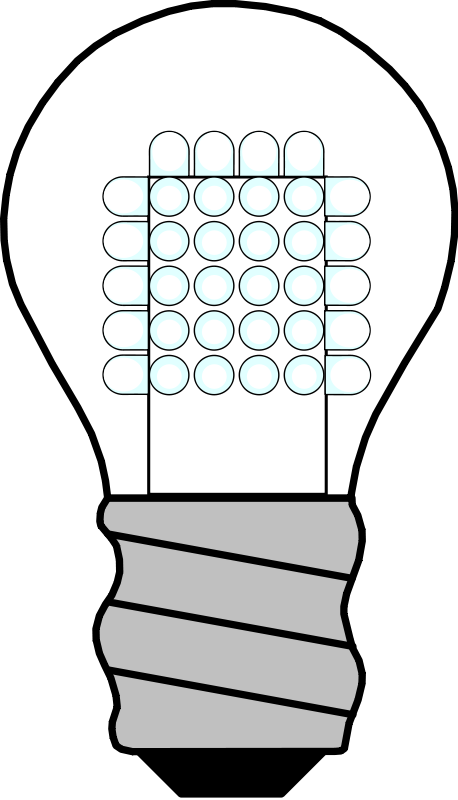
\includegraphics[scale=0.02]{imgs/bulb.png}
 \textbf{Nota} \\
 }%
{\endMakeFramed}

%Work in progress
\newenvironment{workinprogress}{%
  \def\FrameCommand{\colorbox{pink}}%
  \MakeFramed {\FrameRestore}
\lhdbend  \textbf{Work in progress} \\
 }%
{\endMakeFramed}

%Openquestion
\newenvironment{openquestion}{%
  \def\FrameCommand{\colorbox{pink}}%
  \MakeFramed {\FrameRestore}
 \textbf{Domanda aperta} \\
 }%
{\endMakeFramed}

%TODO
\newenvironment{todo}{%
  \def\FrameCommand{\colorbox{pink}}%
  \MakeFramed {\FrameRestore}
 \textbf{TODO} \\
 }%
{\endMakeFramed}

%%%%%%%%%%%%%%%%%%%%%%%%%%%%%%%%
%%%%%%%%%%%% HEADER %%%%%%%%%%%%
%%%%%%%%%%%%%%%%%%%%%%%%%%%%%%%%
\pagestyle{fancy}
% i comandi seguenti impediscono la scrittura in maiuscolo
% dei nomi dei capitoli e dei paragrafi nelle intestazioni
\renewcommand{\chaptermark}[1]{\markboth{#1}{}}
\renewcommand{\sectionmark}[1]{\markright{\thesection\ #1}}
\fancyhf{} % rimuove l'attuale contenuto dell'intestazione
% e del pi\`e di pagina
\fancyhead[LE,RO]{\bfseries\thepage}
\fancyhead[LO]{\bfseries\rightmark}
\fancyhead[RE]{\bfseries\leftmark}
\renewcommand{\headrulewidth}{0.5pt}
\renewcommand{\footrulewidth}{0pt}
\addtolength{\headheight}{0.5pt} % riserva spazio per la linea
\fancypagestyle{plain}{%
\fancyhead{} % ignora, nello stile plain, le intestazioni
\renewcommand{\headrulewidth}{0pt} % e la linea
}


%%%%%%%%%%%%%%%%%%%%%%%%%%%%%%%%
%%%%%%%%%%%% COLORS %%%%%%%%%%%%
%%%%%%%%%%%%%%%%%%%%%%%%%%%%%%%%
\definecolor{code}{gray}{0.3}


%%%%%%%%%%%%%%%%%%%%%%%%%%%%%%%%
%%%%%%%%%%%% NUMBERS %%%%%%%%%%%
%%%%%%%%%%%%%%%%%%%%%%%%%%%%%%%%
\setcounter{tocdepth}{3}
\setcounter{secnumdepth}{3}


%%%%%%%%%%%%%%%%%%%%%%%%%%%%%%%%
%%%%%%%%%%% DOC DATA %%%%%%%%%%%
%%%%%%%%%%%%%%%%%%%%%%%%%%%%%%%%
\title{Appunti di MNO}
\author{Gruppo Informatici Rampanti}
\date{ott 2010 - mag 2011}

\pdfinfo{%
  /Title    (Appunti di MNO)
  /Author   (Andrea Cimino e Lorenzo Muti)
  /Creator  (Andrea Cimino)
  /Producer (Lorenzo Muti)
  /Subject  (MNO)
  /Keywords (MNO)
}


%%%%%%%%%%%%%%%%%%%%%%%%%%%%%%%%
%%%%%%%%%%%%% UTILS %%%%%%%%%%%%
%%%%%%%%%%%%%%%%%%%%%%%%%%%%%%%%
% binary symbols
\newcommand{\modder}{\vdash _{R}}

% vertical gaps
\newcommand{\askip}{\vspace{0.5cm}}
\newcommand{\bskip}{\vspace{1.0cm}}

% various symbols
\newcommand{\qedhere}{\ensuremath{\Box}}
\newcommand{\qed}{\hfill \ensuremath{\Box}}

% substitution
\newcommand{\subst}[2]{^{#1} / _{#2}}

% denotational semantics function names
\newcommand{\bbracket}[1]{\left\llbracket #1 \right\rrbracket}

\newcommand{\aexpr}{\mathcal{A}}
\newcommand{\bexpr}{\mathcal{B}}
\newcommand{\cexpr}{\mathcal{C}}
\newcommand{\Aexpr}[1]{\mathcal{A} \bbracket{#1}}
\newcommand{\Bexpr}[1]{\mathcal{B} \bbracket{#1}}
\newcommand{\Cexpr}[1]{\mathcal{C} \bbracket{#1}}

\newcommand{\semdomset}[1]{(V_{#1})_{\bot}}

% semantic evaluations
\newcommand{\opereval}[3]{\left\langle #1, #2 \right\rangle \rightarrow #3}
\newcommand{\denaeval}[3]{\Aexpr{#1} #2 = #3}
\newcommand{\denbeval}[3]{\Bexpr{#1} #2 = #3}
\newcommand{\denceval}[3]{\Cexpr{#1} #2 = #3}

% rotated sqsubseteqs
\newcommand{\upsqsubseteq}{ $\begin{rotate}{90} $\sqsubseteq$ \end{rotate}$ }
\newcommand{\downsqsubseteq}{ $\begin{rotate}{270} $\sqsubseteq$ \end{rotate}$ }

% Space after paragraph declaration
\makeatletter
\renewcommand\paragraph{\@startsection{paragraph}{4}{\z@}%
  {-3.25ex\@plus -1ex \@minus -.2ex}%
  {1.5ex \@plus .2ex}%
  {\normalfont\normalsize\bfseries}}
\makeatother



% fast theorem and definition
\newcommand{\ftheo}[1]{\colorbox{YellowGreen}{#1}}
\newcommand{\fdefn}[1]{\colorbox{SkyBlue}{#1}}

\theoremstyle{break}
\theoremsymbol{\ensuremath{\clubsuit}}
\theoremseparator{\newline}
\newshadedtheorem{proc}[theo]{Procedura}

% bold math!
\newcommand{\bm}[1]{\mbox{\boldmath{$#1$}}}

\newcommand{\positive}[1]{\textbf{\color{green} +} #1}
\newcommand{\negative}[1]{\textbf{\color{red} -} #1}


\newtheoremlisttype{tab}%
{\begin{tabular*}{\linewidth}{@{}lrl@{\extracolsep{\fill}}r@{}}}%
{##1&##2&##3&##4\\}%
{\end{tabular*}}
\begin{document}
}
\providecommand{\outbpdocument}{\end{document}}
\else
\providecommand{\inbpdocument}{}
\providecommand{\outbpdocument}{}
\fi



\inbpdocument 

%% Bevilacqua 23 Novembre
\chapter{Risoluzione di Sistemi Lineari}

Siano $A \in \mathbb{C}^{n \times n}$ $x,b \in \mathbb{C}^{n}$ e si
supponga che il sistema lineare

$$Ax = b$$
sia consistente (ovvero, ammetta almeno una soluzione).\\ 
I metodi per risolvere il sistema si possono dividere in
\begin{itemize}
\item metodi diretti:
  \begin{itemize}
  \item Gauss
  \item Cholesky (Hermitiane definite positive)
  \item Householder (Maggiori garanzie di stablilit\`a)
  \end{itemize}
\item Metodi iterativi
\end{itemize}

\begin{notes}
  È possibile trattare tutti i metodi diretti come fattorizzazioni
  della matrice dei coefficienti della matrice lineare.
\end{notes}


\section{Propagazione dell'errore}
In un metodo diretto, se non ci fossero errori di rappresentazione dei
dati e di arrotondamento nei calcoli, la soluzione del sistema
verrebbe calcolata esattamente. Invece in un metodo iterativo, anche
nell’ipotesi che non ci siano errori di rappresentazione dei dati e di
arrotondamento nei calcoli, si deve comunque operare un troncamento
del procedimento, commettendo un errore, detto \emph{errore analitico}.\\

Una maggiorazione dell’errore da cui \`e affetta la soluzione può essere
rappresentata da due termini distinti:
\begin{itemize}
\item l'\emph{errore inerente}, dovuto agli errori di rappresentazione dei dati,
che non dipendono dal particolare metodo usato, e
\item l'\emph{errore algoritmico}, dovuto agli errori di arrotondamento nei calcoli,
che dipende dal metodo usato, ma non dagli errori sui dati.
\end{itemize}

Lo studio dell’errore inerente può essere fatto perturbando i dati ed
esaminando gli effetti indotti sulla soluzione.

\begin{theo}[Numero di condizionamento di $A$]
Siano $\delta A \in \mathbb{C}^{n \times n}$ e $\delta b \in
\mathbb{C}^n$ rispettivamente la matrice e il vettore delle
perturbazioni sui dati del sistema, dove $b \neq 0$ e sia $|| \cdot
||$ una qualunque norma indotta. Se $A$ non \`e singolare e se $||
A^{-1}|| \; || \delta A|| < 1$ allora anche la matrice $A + \delta A$
\`e non singolare. Indicata con $x + \delta x$ la soluzione del sistema perturbato
$$(A + \delta A) (x + \delta x) = b + \delta b$$

risulta 
$$ \frac{||\delta x||}{||x||} \leq \mu(A)
\frac{ \frac{|| \delta A||}{||A||} + 
\frac{|| \delta b||}{||b||}}{1 - \underbrace{\mu(A) \frac{||\delta A||}{||A||}}_{<1}}
$$
in cui $ \mu(A)  = ||A|| \; ||A^{-1}|| $ \`e detto \emph{numero di
  condizionamento} della matrice $A$
\end{theo}

Si osservi che il numero di condizionamento \`e sempre maggiore o
uguale a 1. Inoltre se $\mu(A)$ assume valori piccoli, allora piccole
perturbazioni sui dati inducono piccole perturbazioni sulla soluzione
e la matrice del sistema \`e ben condizionata.\\
Un metodo risulta più \emph{stabile} di un altro se \`e meno sensibile
agli errori indotti dai calcoli. Lo studio della stabilit\`a di un
metodo perde di significativit\`a quando il problema \`e fortemente mal
condizionato, poich\'e in questo caso l’errore inerente prevale
sull’errore algoritmico.




\section{Fattorizzazione}
I metodi diretti che vedremo utilizzano una fattorizzazione della
matrice A, nel prodotto di due matrici B e C, facilmente invertibili.
$$ A = BC $$
Possiamo dunque riscrivere il sistema, e la sua soluzione si riduce
alla risoluzione di due sottoproblemi:
$$ BCx = b \qquad
\left\{ 
  \begin{array}{l}
  By = b\\
  Cx = y                                         
  \end{array}
\right.
$$
$B$,$C$ possono appartenere alle seguenti classi:
\begin{itemize}
 \item Triangolari (Si risolve per sostituzione
   all'indietro). $O(n^2)$ operazioni.
 \item Unitarie (Sono facili da invertire). Infatti
     $Qx =b \rightarrow x =Q^{H}b$. $O(n^2)$ operazioni.
\end{itemize}

Vedremo le seguenti 3 fattorizzazioni classiche. \\

$A = LU$
\begin{itemize}
\item $L$ \`e triangolare inferiore (Lower) con diagonale unitaria ($l_{ii}=1$)
\item $U$ \`e triangolare superiore (Upper)
\item associata al metodo di Gauss.
\end{itemize}

$A = LL^{H}$
\begin{itemize}
\item $L$ \`e triangolare inferiore con elementi positivi sulla
  diagonale ($\mathbb{R} \ni l_{ii}>0$)
\item associata al metodo di Cholesky.
\end{itemize}

$A = QR$
\begin{itemize}
\item $Q$ unitaria 
\item $R$ triangolare superiore
\item associata al metodo di Householder.
\end{itemize}

Se la matrice $A$ \`e reale, le matrici delle tre fattorizzazioni, quando
esistono, sono reali.\\
Il costo computazionale della fattorizzazione \`e $O(n^3)$ operazioni,
mentre il costo computazionale della risoluzione dei sistemi \`e
$O(n^2)$ operazioni.\\
La fattorizzazione $QR$ esiste per ogni matrice $A$, mentre non sempre \`e
possibile ottenere le fattorizzazioni $LU$ e $LL^H$. Valgono infatti i
seguenti teoremi.

\paragraph{Fattorizzazione LU}
\begin{theo}[Esistenza della fattorizzazione $A=LU$]\label{th:LU}
Sia $A$ una matrice di ordine $n$ e siano $A_k$ le sue sottomatici
principali di testa di ordine $k$. Se $A_k$ \`e non singolare per
$k=1,\ldots,n-1$ allora esiste ed \`e \emph{unica} la fattorizzazione
$LU$ di $A$.
\end{theo}

\begin{thproof}
  Per induzione su $n$
  \begin{itemize}
  \item $n=1$\\
    \[\begin{array}{ccc}
      a_{11} = & 1 \cdot & a_{11} \\ 
      A        & L       & U
    \end{array}\]
    (oppure $a_{11}$ potrebbe essere uguale a $0$).
 \item $n>1$\\
\[
A = \left |
\begin{array}{c|c}
A_{n-1} & \mathbf{d} \\ \hline
\mathbf{c}^{H} &  \alpha
\end{array}
\right | = \left |
\begin{array}{c|c}
L_{n-1} & \mathbf{0} \\ \hline
\mathbf{u}^{H} &  1
\end{array}
\right |
\cdot
\left |
\begin{array}{c|c}
U_{n-1} & \mathbf{v} \\ \hline
\mathbf{0}      & \beta
\end{array}
\right |
\]
Otteniamo le sequenti equazioni:
\[\left\{
  \begin{array}{ll}
    A_{n-1} = L_{n-1} \cdot U_{n-1} & (1) \\
    d = L_{n-1} \cdot v           & (2)  \\
    c^{H} = u^{H} \cdot U_{n-1} \quad \rightarrow \quad 
    c = U^{H}_{n-1} \cdot u \quad  & (3) \\
    \alpha = u^{H} \cdot v + \beta &(4) \\
  \end{array}
\right.\]
Da cui traiamo le seguenti:
\begin{itemize}
\item $(1)$ essendo $L_{n-1}$ triangolare superiore $det(L_{n−1}) =
  \Pi_{i=0}^{n-i} l_{ii} = 1$ allora $det (U_{n-1}) = det(A_{n-1})$ che
  per ipotesi \`e diverso da zero. Quindi esistono le inverse di $L$ e $U$
  e i seguenti valori sono determinati univocamente.
\item $(2)$ $v = L^{-1}_{n-1} \cdot d$ 
\item $(3)$ $u = (U_{n-1}^{H})^{-1} \cdot c$
\item $(4)$ $\beta = \alpha - u^{H} \cdot v$ 
\end{itemize}
\end{itemize}
\end{thproof}

Se cade l'ipotesi del teorema perdiamo l'unicit\`a, possiamo non avere
alcuna fattorizzazione o averne più di una.
\begin{example}[Fattorizzazione non unica]
\[ 
A = 
\begin{pmatrix}
0 & 1 \\
0 & 2 
\end{pmatrix}
= \underbracket{
\begin{pmatrix}
1 & 0  \\
l & 1 
\end{pmatrix}}_{L}
\cdot \underbracket{
\begin{pmatrix}
0 & 1  \\
0 & u 
\end{pmatrix}}_{U}
\]
esistono infinite combinazioni per cui vale $l+u=2$.
\end{example}

\begin{theo}
  Per ogni matrice A, esiste una matrice di permutazione $\Pi$ per cui
  si può ottenere la fattorizzazione $LU$ di $\Pi A$, cio\`e
  $$\Pi A = LU$$
\end{theo}

%  TODO COSA È QUESTA??
% $$
% \[
% \left(
% \begin{array}{c|ccc}
%   a_{11} & 1 & 1 & 1 \\ \hline \\[-9pt]
%   0 & \multicolumn{3}{c}{\multirow{4}{*}{\Huge $C$}} \\[-4pt]
%   \vdots & \\
%   0 &
% \end{array}
% \right)
% \]
% $$

\paragraph{Fattorizzazione $LL^{H}$}
\begin{theo}[Esistenza fattorizzazione $LL^{H}$]\label{th:esistenza-LL}
Sia A una matrice hermitiana definita positiva, allora esiste ed \`e
unica la fattorizzazione $LL^H$ di A.
\end{theo}

\begin{thproof}
  con $l_{ii} > 0$. \\
  Per il teorema \ref{richiamibevilacqua:theo01},
  $A$ ha le sottomatrici $A_k$ con $det(A_k) > 0$ e quindi per il
  teorema \ref{th:LU} esiste unica la fattorizzazione (per evitare
  confusione rinominiamo L con M):
  $$ A = M \cdot U $$
  in cui ricordiamo che M \`e triangolare inferiore $m_{ii}=1$ e U \`e
  triangolare superiore. Possiamo scomporre ancora:
  $$ A = M \cdot \underbracket{D \cdot R}_{U}$$
  Con D matrice diagonale i cui elementi principali sono quelli di U,
  e R triangolare superiore con $r_{ii} = 1$.

  $$
  \underbracket{
    \begin{pmatrix}
      u_{11} & u_{12}  \\
      0     & u_{22}
    \end{pmatrix}}_{U} = \underbracket{
    \begin{pmatrix}
      u_{11} & 0  \\
      0     & u_{22}
    \end{pmatrix}}_{D} \underbracket{
    \begin{pmatrix}
      1 & \frac{u_{12}}{u_{11}} * \\
      0 & 1
    \end{pmatrix}}_{R}
  $$
* \`e possibile solo se $det(A)\neq0$ ed \`e effetivamente così nel nostro
caso, infatti $\left\{
  \begin{array}{l}
    det(U) \neq 0 \\
    det(A) > 0
  \end{array}
\right.$

Dalla propriet\`a delle hermitiane $A^{H} = A$ otteniamo:
$$ \underbracket{R^{H}}_{L}\underbracket{D^{H} M^{H}}_{U} =
\underbracket{M}_{L}\underbracket{DR}_{U} $$ dato che abbiamo da entrambi i lati
la fattorizzazione LU, dalla sua unicit\`a otteniamo: 
\[\begin{array}{l}
  R^{H} = M \; \Rightarrow \; M^{H} = R \\
  DR = D^{H}M^{H}= D^{H}R  \Rightarrow  D = D^{H}
\end{array}\]
Sappiamo quindi che $d_{ii}  = \overline{d}_{ii}$, quindi $D \in
\mathbb{R}$.\\

Vogliamo ora dimostrare che D \`e hermitiana definita positiva, partiamo
dalla definizione:
$$ x^{H}Dx = \underbracket{x^{H} M^{-1}}_{y^{H}}
\underbracket{MDM^{H}}_{A} \underbracket{(M^{H})^{-1} x}_{y} = y^{H}Ay
\underbracket{>}_{A\;def\;pos} 0 $$
Quindi possiamo concludere che anche $D$ \`e diagonale ed hermitiana
definita positiva, ed avendo solo autovalori positivi, avr\`a $d_{ii}>0$.\\

Esiste allora un’unica matrice diagonale $F$ ad elementi principali
reali e positivi, tale che $D = F^2$, e quindi $F =
diag\{\sqrt{d_{ii}}\}$. Da cui possiamo ricavare:

$$ A = MDR = \underbracket{M F} \underbracket{F^H M^H} = LL^H $$

Notare che la fattorizzazione di Cholesky \`e \emph{caratterizzante}: se
A \`e fattorizzabile $LL^H$ allora \`e hermitiana definita positiva.
\end{thproof}


\paragraph{Fattorizzazione QR}\label{fatt:QR}
A differenza della fattorizzazione $LU$ e $LL^H$ , la fattorizzazione $QR$ di
una matrice A non \`e unica. 

\begin{observation}
  Se Q e R esistono, non sono uniche.
\end{observation}
\begin{thproof}
  Se $A = QR = Q \underbracket{D D^{-1}}_{I} R$  \\
  e scegliamo $D$ come matrice diagonale e unitaria, quindi con $|d_{ii}| = 1$, abbiamo
  $$ D D^H = 
  \begin{array}{|ccc|}
    \ddots & & \\
    & d_{ii} \cdot \overline{d}_{ii} & \\
    & & \ddots
  \end{array}
  = I $$
e possiamo scrivere 
$$ A = QR = \underbracket{Q D}_{\text{unit}}
\underbracket{D^{H} R}_{\text{tri. sup}} = Q_1 R_1 $$
quindi abbiamo ottenuto un'altra fattorizzazione.\\
Le matrici D vengono dette \emph{matrici di fase} ed solo con queste
che la fattorizzazione non \`e unica, quindi possiamo dire che la
fattorizzazione QR \`e unica a meno di matrici di fase.
\end{thproof}


La determinazione delle matrici della fattorizzazione di A viene 
generalmente effettuata nei due modi seguenti:
\begin{itemize}
\item applicando alla matrice A una \emph{successione di matrici
    elementari}  (metodo di Gauss, metodo di Householder);
\item con \emph{tecniche compatte} (metodo di Cholesky).
\end{itemize}

\section{Metodo di Gauss}
Nel metodo si ricava una incognita da una delle equazioni e si
sostituisce in tutte le altre, ripetendo il procedimento fino a
trovare la soluzione (nella variante classica impone una certa
strategia nella risoluzione).\\
Il cambiamento della matrice dovuto alla sostituzione dei coefficienti
può essere espresso come la moltiplicazione per una matrice E:
$$ E A^{(1)} = A^{(2)} $$

Dove  $A^{(1)}$ e $A^{(2)}$ sono la matrici prima e dopo la sostituzione.
La matrice $E$ \`e detta \emph{elementare} ed ha diagonale unitaria e la
prima colonna diversa da zero.

\[
E = \left |
\begin{array}{ccccc}
1      &   &  & \multicolumn{2}{c}{\multirow{2}{*}{\huge $0$}}      \\
x_2    & 1 &  &                                                     \\
\vdots & \multicolumn{2}{c}{\multirow{2}{*}{\huge $0$}} & \ddots &  \\
x_n    &   &  & &1
\end{array}
\right |
\]

Facendo i passi sequenti avremo:
$$ E^{(S)} \ldots E^{(2)} \cdot E^{(1)} \cdot A^{(1)} = U $$
con $U$ triangolare superiore.
Ora portando al secondo membro:
$$ A = A^{(1)} = \underbracket{(E^{(S)} \ldots E^{(1)})^{-1}}_{L} U $$


$$ A^{(n)} = E^{(n-1)}\ldots E^{(2)} E^{(1)}A$$
\begin{defn}[Matrice Elementare]
Siano $\sigma \in \mathbb{R}$ e $u,v \in \mathbb{C}^n, u,v, \neq
0$. Si definisce \emph{matrice elementare}:
$$ E(\sigma, \mathbf{u},\mathbf{v}) = 
   I - \sigma \mathbf{uv}^{H} $$


\[\left | \begin{array}{ccccc}
    1  &   &  & \multicolumn{2}{c}{\multirow{2}{*}{\huge $0$}}      \\
       & 1 &  &                                                     \\
    \multicolumn{2}{c}{\multirow{2}{*}{\huge $0$}}  &   & \ddots &  \\
       &  & & & 1
\end{array} \right |
-\sigma
\left | \begin{array}{c}
    x \\
    x \\
    \vdots \\
    x
\end{array} \right |
|x \; x \; \cdots \; x|
\]
\end{defn}

\begin{notes}\textbf{Perch\'e calcola questi autovalori come se la diade fosse singolare?}\\
  $\sigma u v^{H}$ \`e detta \emph{diade} ed ha rango $\leq 1$,
  TODO???$det(\sigma u v^{H}) = 0$.\\
I suoi autovalori sono:
\begin{itemize}
\item $\lambda_1 = 0$  (molteplicita $n-1$)
\item $\lambda_2 = \sigma v^{H} u$   (molteplicit\`a $1$)
\end{itemize}

Quindi gli autovalori di $E$ sono:
$\left\{ 
 \begin{array}{ll}
 1-0 = 1            & \text{molt. n-1} \\
 1 - \sigma v^{H} u & \text{molt. 1}
\end{array}
\right.$\\
dai quali ricaviamo il determinante di E: $det(E) = 1 (1 - \sigma v^H
u) \neq 0$.\\
Quindi $E$ \`e invertibile se e solo se $\sigma v^{H}u \neq 1$, infatti
questa condizione \`e l'ipotesi del seguente teorema che ci permette di
calcolare l'inversa di una matrice elementare.
\end{notes}

La classe delle matrici elementari non singolari \`e chiusa rispetto
all'operazione di inversione. Vale infatti il seguente teorema.

\begin{theo}[Invertibilit\`a matrici elementari]
\label{th:eleminversa}
  Ogni matrice elementare $E(\sigma, \mathbf{u, v})$ per cui $\sigma
  \mathbf{v}^H \mathbf{u} \neq 1$ \`e invertibile e la sua inversa \`e
  ancora una matrice elementare della forma e $E(\tau, \mathbf{u, v}),
  \tau \in \mathbb{C}$.
\end{theo}

\begin{thproof}
Se $\sigma=0$ la tesi \`e ovvia. Per $\sigma \neq 0$ dimostriamo che
esiste un $\tau$ tale che:
\[\begin{array}{ll}
 (I - \sigma uv^{H})(I - \tau u v^{H}) = I \\
 \cancel{I} - (\sigma + \tau) uv^{H} + \sigma \tau u 
 \underbracket{v^{H} u}_{scalare} v^{H} = \cancel{I} \\
 \underbracket{(-\sigma - \tau +  \sigma \tau v^{H}
   u)}_{\text{scalare}} \underbracket{uv^{H}}_{\text{matrice}} = 0 
\end{array}\]

Per non cadere nel caso in cui $E=I$, poniamo che ne $u$ ne $v$ siano
nulli. Allora possiamo concludere che
\[\begin{array}{ll}
 - \sigma - \tau + \sigma\tau v^{H} u = 0 \\
 \tau(-1 + \sigma v^{H}u) = \sigma \\
 \tau = \frac{\sigma}{\sigma v^{H}u-1} 
\end{array}\]
che esiste perch\'e per ipotesi $\sigma v^{H}u \neq 1$.
\end{thproof}

Vogliamo usare le matrici elementari per il metodo Gauss, e quindi ci
chiediamo se esista una $E$ tale che $A^{(2)} = E A^{(1)}$, questo ci \`e
garantito dal teorema seguente.

\begin{theo}\label{th:elem}
  Siano $x,y \in \mathbb{C}^n$, $x,y \neq \mathbf{0}$. Esistono matrici
  elementari non singolari $E(\sigma, u, v)$ tali che 
  $$ E(\sigma, u, v)x = y $$
\end{theo}

\begin{thproof}
 Vogliamo mostrare che:
  $$ (I - \sigma uv^{H}) x = y$$
  $$ x - \sigma u v^{H} x = y $$
  $$ \sigma u = \frac{x -y} {v^{H}x}$$
  Quindi la prima condizione \`e che $v^{H}x \neq 0$.\\ 
  Inoltre per avere $E$ invertibile \`e necessario che $\sigma
  v^{H}u \neq 1$, da cui

  $$ v^{H}\underbracket{\sigma u} = v^{H} \frac{x - y}{v^{H}x} = 
  \frac{v^{H}x}{v^{H}x} - \frac{v^{H}y}{v^{H}x}
  = 1 - \frac{v^{H}y}{v^{H}x} \neq 1 $$ 
  $$ \frac{v^{H}y}{v^{H}x} \neq 0 \quad \Rightarrow \quad v^{H}y \neq 0 $$
  Quindi per ottenere la matrice E basta rispettare il seguente sistema:
  $$ v:  \left\{
    \begin{array}{ll}
      v^{H} x \neq 0 & \text{esistenza}\\
      v^{H} y \neq 0 & \text{invertibilit\`a}
    \end{array}
  \right.
  $$
\end{thproof}

\section{Matrici Elementari di Gauss}
Vediamo ora quali matrici elementari sono adatte per il metodo di Gauss.\\
Sia $\mathbf{x}$, con $x_1 \neq 0$. Si vuole determinare una matrice

$$ M = E(\sigma, \mathbf{u},\mathbf{e}_1 ) = I - \sigma \mathbf{u} {\mathbf{\underbracket{\mathbf{e}_1}_{v}}}^H
\qquad 
\mathbf{e}_1 = | \; 1 \; 0 \; \cdots \; 0 \; |^{T} 
$$
tale che
$$ M\mathbf{x} = \underbracket{x_1 \mathbf{e}_1}_{\mathbf{y}} = 
| \; x_1 \; 0 \; \cdots \; 0 \; |^T
$$
cio\`e "proietti" la prima componente del vettore $\mathbf{x}$.
Dobbiamo quindi trovare  $\sigma$ ed  $\mathbf{u}$ per cui valga questa
condizione.
\paragraph{Esistenza}
 Per stabilire l'esistenza di $M$: sappiamo che vale la condizione
% \[\left\{
% \begin{array}{ll}
% \mathbf{e}_1^{H} \mathbf{x} = x_1 \neq 0                             \\
% \mathbf{e}_1^{H} x_1 \mathbf{e}_1 = x_1 \neq 0                        \\
% \end{array}
% \right.
% \quad \Longrightarrow \quad
% x_1 \neq 0
% \]
  $$\mathbf{e}_1^{H} \mathbf{x} = x_1 \neq 0$$
 Ed il teorema \ref{th:elem} ci dice che questa condizione \`e sufficiente
 per l'esistenza.\\
Quindi
$$ \sigma \mathbf{u} = \frac{\mathbf{x}-\mathbf{y}}{\mathbf{v}^{H}\mathbf{x}}
=  \frac{\mathbf{x} - x_1\mathbf{e}_1}{\mathbf{e}^{H}_1\mathbf{x}}
=  \frac{\mathbf{x} - x_1\mathbf{e}_1}{x_1} = \frac{1}{x_1}
\begin{array}{|l|}
  0                                               \\
  x_2                                             \\ 
  \vdots                                          \\ 
  x_n
\end{array} 
=
\begin{array}{|l|}
  0                                               \\
  \frac{x_2}{x_1}                                 \\ 
  \vdots                                          \\ 
  \frac{x_n}{x_1}
\end{array} $$

 
La matrice $M^{(1)}$ \`e perció:
\[M^{(1)} = 
\begin{pmatrix}
1                &   &        &                   \\
-\frac{x_2}{x_1} & 1 &        &                   \\
\vdots           &   & \ddots &                   \\
-\frac{x_n}{x_1} &   &        & 1 
\end{pmatrix}\]

\paragraph{Matrice inversa}
 La matrice $M$ risulta invertibile sfruttando \ref{th:eleminversa}, in quanto
$$ \sigma \mathbf{e}_1^{H}\mathbf{u} = 0$$

Possiamo quindi calcolare la  sua inversa, partendo dal valore di $\tau$:
$$ \tau = \frac{\sigma}{\sigma \underbracket{\mathbf{v}^{H}\mathbf{u}}_{=0}-1}= -\sigma$$
Nel caso del metodo di Gauss $v^{H}u = 0$ dato che $v^{H}=|1 \; 0 \; \ldots
\; 0|$ e $u = |0 \; x \; \ldots \; x|^{-1}$.\\
Quindi in generale una matrice inversa della elementare di Gauss \`e data da
$$ M^{-1} = I + \sigma \mathbf{u} \mathbf{e}_1^{H} $$

nel nostro caso:
\[(M^{(1)})^{-1} = 
\begin{pmatrix}
1               &   &        &                   \\
\frac{x_2}{x_1} & 1 &        &                   \\
\vdots          &   & \ddots &                   \\
\frac{x_n}{x_1} &   &        & 1 
\end{pmatrix}\]

Le matrici elementari hanno la propriet\`a di trasformare un
qualunque vettore non nullo in un vettore con al più una componente
diversa da zero. Quindi possiamo sfruttarle per trasformare in forma
triangolare superiore una matrice, moltiplicandola successivamente per
opportune matrici elementari.\\
Al $k$-esimo passo, posto $a^{(k)}_{kk} \neq 0$ si considera il vettore 
$$ m^{(k)} = | \; \underbracket{0 \; \cdots \; 0}_{k\text{ componenti}} m_{k+1,k} \; \cdots \; m_{nk} \; |^T $$
dove $m_{ik} = a^{(k)}_{ik} / a^{(k)}_{kk}$ con $i = k+1,\ldots,n$ da
cui ricaviamo 

\[ E^{k} = E(1,m^{(k)}, e_k) = M^{(k)} =
\begin{pmatrix}
1 &        &            &        & \\
  & \ddots &            &        & \\
  &        & 1          &        & \\
  &        & -m_{k+1,k} &        & \\
  &        & \vdots     & \ddots & \\
  &        & -m_{nk}    &        & 1 
\end{pmatrix}\]

Poniamo ora 
$$ U = A^{(n)} = M^{(n-1)} \ldots M^{(2)} M^{(1)} A $$

Possiamo utilizzare l'inversione delle $M$, ottenendo quindi
$$ \underbracket{(M^{(1)})^{-1} \ldots (M^{(n-2)})^{-1} (M^{(n-1)})^{-1}}_{L} U = A $$
\[ L = (M^{(1)})^{-1} \ldots (M^{(n-1)})^{-1} = 
\begin{pmatrix}
1      &        &           &        &           & \\
m_{21} & \ddots &           &        &           & \\
       & \ddots & 1         &        &           & \\
\vdots &        & m_{k+1,k} &        &           & \\
       &        & \vdots    & \ddots & \ddots    & \\
m_{n1} & \cdots & m_{nk}    & \cdots & m_{n,n-1} & 1
\end{pmatrix}\]



\begin{figure}[h]
 \centering
 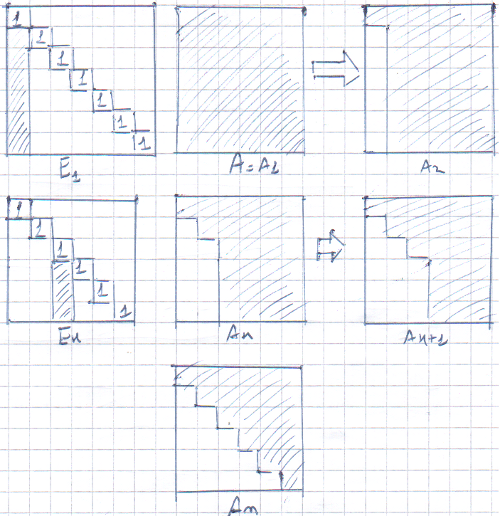
\includegraphics[width=0.40\textwidth]{./imgs/lu.png}
 % lu.png: 500x516 pixel, 150dpi, 8.47x8.74 cm, bb=0 0 240 248
 \caption{Passi della trasformazione $LU$ per mezzo di matrici elementari di Gauss}
\end{figure}

% Vediamo il secondo passo di questo processo:
% \[\begin{array}{cccc}
% M^{(2)} &A^{(2)} &= &A^{(3)} \\
% % TODO verificare come \`e fatta questa matrice
% \begin{pmatrix}
% 1      & 0      & 0 & \ldots & 0                  \\
% 0                                                 \\
% 0                                                 \\
% \vdots                                            \\
% 0                
% \end{pmatrix}
% &
% \begin{pmatrix}
% x      & x      & x & \ldots & x                  \\
% 0      & x      & x & \ldots & x                  \\
% 0      & x      & x & \ldots & x                  \\
% \vdots & x      & x & \ldots & x                  \\
% 0      & x      & x & \ldots & x
% \end{pmatrix}
% &
% &\begin{pmatrix}
% x      & x      & x & \ldots & x                  \\
% 0      & x      & x & \ldots & x                  \\
% 0      & 0      & x & \ldots & x                  \\
% \vdots & \vdots & x & \ldots & x                  \\
% 0      & 0      & x & \ldots & x
% \end{pmatrix}
% \end{array}\]


Quindi il procedimento consiste nel prodotto di n matrici triangolari
inferiori con elementi diagonali uguali a 1, ed il risultato \`e ancora
una matrice di questa forma, quindi compatibile con la nostra
definizione di matrice $L$ del metodo $LU$.

\begin{example}
Per n = 4
$$ (M^{(1)})^{-1} (M^{(2)})^{-1}(M^{(3)})^{-1} = 
\begin{pmatrix}
  1      &        &        & \\
  m_{21} & 1      &        & \\
  m_{31} &        & 1      & \\
  m_{41} &        &        & 1
\end{pmatrix}
\begin{pmatrix}
  1      &        &        & \\
         & 1      &        & \\
         & m_{32} & 1      & \\
         & m_{42} &        & 1
\end{pmatrix}
\begin{pmatrix}
  1      &        &        & \\
         & 1      &        & \\
         &        & 1      & \\
         &        & m_{43} & 1
\end{pmatrix} =
\begin{pmatrix}
  1      &        &        & \\
  m_{21} & 1      &        & \\
  m_{31} & m_{32} & 1      & \\
  m_{41} & m_{42} & m_{43} & 1
\end{pmatrix} = L
$$
\end{example}

L'elemento $a_{kk}$ della matrice $A^{(k)}$, detto \emph{pivot} al
k-esimo passo, \`e per ipotesi diverso da zero e dato che $A^{(k)}$ \`e
triangolare superiore per \ref{triangolari}
$$ \det(A_k) = a^{(1)}_{11} \cdot \ldots \cdot a^{(k)}_{kk} \neq 0 $$
quindi $A^{(k)}$, detta minore principale di testa, \`e non singolare.

% TODO Cosa avr\`a voluto dire?
% $$ A^{(k)} = M^{(k-1)} \ldots M^{(1)} A^{(1)} $$
% La sottomatrice superiore sinistra () $B$
% $k \times k$, viene raggiunta quanto si arriva ad usare $M^{(k-1)}$, 
% allora sappiamo che il determinante di $B$ \`e il prodotto degli
% $a^i_{ii}$ per \ref{triangolari}
% Il Minore principale di testa \`e uguale al prodotto dei minori principali di testa di 
% $$ M^{(k-1)} \ldots M^{(1)}A^{(1)} $$
% Quindi abbiamo $a_{kk}^{(k)} = det A_k \neq 0 $ (gli M sono nulli)

%% 7 Dicembre
\section{Matrici elementari di Householder}
\label{sec:householder}
% TODO
% $P^{(i)}$ matrici elementari \emph{unitarie} perche vogliamo $Q$ unitaria.
% Inoltre $P^{(i)}$ unitaria Hemitiane \\
% Avremo 
% $Px = [ \alpha, 0 ,0,\ldots, 0] = \alpha e_1$
Il procedimento di fattorizzazione della matrice A con matrici di
Householder \`e sempre applicabile. Queste matrici ci servono per
costruire la fattorizzazione $QR$.
$$ A = \underbracket{Q}_{\text{unitaria}}\cdot\underbracket{R}_{\text{tr. sup.}} $$

Dobbiamo trovare una matrice elementare  $P$ unitaria tale che
$$ P_{n-1} \ldots P_{1} \cdot A = R$$
$$ A = \underbracket{(P_{n-1}\ldots P_{1})^{-1}}_{Q}R $$

\begin{defn}[Matrice elementare di Householder]
  Una matrice elementare hermitiana
  $$ P = I - \beta \mathbf{\mathbf{v} \mathbf{v}}^H $$
  con $\beta \in \mathbb{R}$ e $\mathbf{v} \in \mathbb{C}^n,\mathbf{v} \neq 0$, \`e detta
  \emph{matrice di Householder} se \`e unitaria, cio\`e se $P^H P = P P^H = I$.
\end{defn}

Per ogni vettore $\mathbf{x} \in \mathbb{C}^n$, con $\mathbf{x} \neq 0$, si può
determinare una matrice di Householder $P$ tale che 
 $$ P\mathbf{x} = \alpha \mathbf{e}_1 $$ 
dove $\alpha$ \`e una opportuna costante e $\mathbf{e}_1$ \`e il primo vettore della base canonica. Nel metodo, $x$ assumerà i valori delle colonne di $A$, dalla prima all'$n$-esima, che si vorranno trasformare.

\begin{property}
  La matrici unitarie godono della seguenti propriet\`a:
  \begin{itemize}
  \item $$ U^{-1} = U^{H}$$
  \item moltiplicare per una matrice unitaria non cambia la norma 2
    $$ || U\mathbf{x} ||_{2} = || \mathbf{x} ||_{2} \quad \text{vettori}$$
    $$ || UM ||_{2} = || M ||_{2} \quad \text{matrici}$$
    Per quanto riguarda le norme di vettori infatti,
    ricordando che 
    $$||\mathbf{x}|| \defeq \sqrt{\mathbf{x}^{H}\mathbf{x}} =
    \sqrt{\displaystyle \sum_{i}^{n} |x_i|^{2}}$$
    otteniamo
    $$ || U\mathbf{x} ||_{2} = \sqrt{(U\mathbf{x})^{H} U\mathbf{x}} =
    \sqrt{\mathbf{x}^{H}U^{H}U\mathbf{x}} = \sqrt{\mathbf{x}^{H}\mathbf{x}} =
    ||\mathbf{x}||_{2}$$
    Invece per le matrici consideriamo la norma indotta (spettrale) $\rho$.
    Ricordando che
    $$||M||_2 \defeq \sqrt{\rho(M^{H}M)}$$
    otteniamo

    $$ || UM ||_{2} = \sqrt{\rho\left((UM)^{H} UM \right)} = \sqrt{\rho(M^{H}U^{H}UM)} = \sqrt{\rho(M^{H}M)} = ||M||_{2} $$
    Quindi la matrice unitaria \`e una trasformazione che conserva le lunghezze:
    una \emph{isometria}
\end{itemize}
\end{property}

Quindi, nel procedimento che useremo, conserveremo le lunghezze, e questo
\`e importante per la stabilit\`a.\\

\paragraph{Condizioni per $\beta$}
Dal fatto che P \`e unitaria e hermitiana ricaviamo:
$$ I \underbracket{=}_{unit.} PP^{H} \underbracket{=}_{herm.} PP = 
(I - \beta \mathbf{v}\mathbf{v}^{H})(I - \beta \mathbf{v}\mathbf{v}^{H}) = 
\cancel{I} - 2\beta \mathbf{v}\mathbf{v}^{H} + \beta^{2} \mathbf{v} \underbracket{\mathbf{v}^{H}\mathbf{v}}_{scalare}\mathbf{v}^{H} = 
\cancel{I} $$
%\[\begin{array}{ll}
In sostanza dobbiamo rispettare la condizione 
$$ \beta(-2\mathbf{v}\mathbf{v}^{H} + \beta \mathbf{v}^{H}\mathbf{v} \mathbf{v}\mathbf{v}^{H}) = 0 $$
Ponendo la condizione $\beta \neq 0$
   $$( -2 + \beta \mathbf{v}^{H}\mathbf{v}) \mathbf{v}\mathbf{v}^{H} = 0$$ 
e  ponendo $\mathbf{v} \neq 0$, come richiesto dalla
   definizione di elementare di Householder, otteniamo
  $$ \beta = \frac{2}{\mathbf{v}^{H}\mathbf{v}} = 
  \frac{2}{||\mathbf{v}||^{2}_{2}}
    $$
% &
  % \mathbf{0} \text{ (caso banale), come da definizione} \\ \\
  % \beta = \frac{2}{\mathbf{v}^{H}\mathbf{v}} = \frac{2}{||\mathbf{v}||^{2}_{2}} &
  % \text{condizione per unitariet\`a}
%\end{array}\]

\paragraph{Condizioni per $\alpha$}
Inoltre dato che $P\mathbf{x} = \alpha \mathbf{e}_1$ e P \`e unitaria abbiamo la seguente condizione su $|\alpha|$
$$ ||\mathbf{x}||_2 = ||P\mathbf{x}||_2 = || \alpha e_{1}||_2 = |\alpha| $$

Inoltre dalle propriet\`a delle hermitiane risulta $ \mathbf{x}^{H}P\mathbf{x} \in
\mathbb{R}$, da cui:
$$ \mathbb{R} \ni \mathbf{x}^{H}P\mathbf{x} = \mathbf{x}^{H} \alpha \mathbf{e}_1 = \overline{x}_1 \alpha = \ldots $$
                                                               \\
Ora esprimiamo
\[\begin{array}{rll}
 \alpha         & = |\alpha| &(\cos(\varphi) + i \sin (\varphi)) \\
 x_1            & = |x_1| &(\cos(\psi)      + i \sin (\psi))  \\
 \overline{x_1} & = |x_1| &(\cos(-\psi)    + i \sin (-\psi))
\end{array}\]
Ricordando dalla trigonometria che
$$
\begin{array}{l}
\mathbb \mathrm{sen} \, (\alpha - \beta)=\mathrm{sen} \, \alpha \, \cos\beta - \cos\alpha \, \mathrm{sen} \, \beta \\
\mathbb \cos(\alpha - \beta)=\cos\alpha \, \cos\beta + \mathrm{sen} \, \alpha \, \mathrm{sen} \, \beta   
\end{array}
$$
otteniamo
$$ \ldots = |x_1| |\alpha| (\cos(\varphi - \psi) + i \sin(\varphi - \psi))$$
% x_1 x_2 .... x_n  \alpha
%                     0
%                     0
%                     0
%                     0
%                     0
Affinch\'e questo numero sia reale \`e necessario annullare la sua parte
immaginaria. \\
$$ \sin(\varphi - \psi) = 0 
\quad \text{da cui due possiblit\`a} \quad
\left\{
\begin{array}{ll}
  \varphi = \psi               & (1) \\
  \varphi = \pi  + \psi        & (2) \\
\end{array}
\right.
$$
Poniamo $\theta = (\cos(- \psi) + i \sin (-\psi))$ ed esprimiamolo in
funzione di $\mathbf{x}$ come $\theta = \frac{x_1}{|x_1|}$, ed esprimiamo a sua
volta $\alpha$ in funzione di $\theta$. In pratica $\theta$ \`e il \emph{versore}, che rappresenta la direzione di $x$. Vogliamo che $\alpha$ abbia la stessa
direzione di $x$, oppure quella opposta. Vediamo i vincoli su $\alpha$
delle precedenti condizioni:
\[\begin{array}{ll}
  \alpha  = |\alpha| \theta    & (1) \\
  \alpha  = |\alpha| (-\theta) & (2)
\end{array}\]

\paragraph{Condizioni per $\mathbf{v}$}
A questo punto manca da trovare $\mathbf{v}$ tale che $\beta = \frac{2}{|| \mathbf{v} ||^2_2}$
\[\begin{array}{lll}
 P\mathbf{x} &= \alpha \mathbf{e}_1 \\
 (I - \beta \mathbf{v}\mathbf{v}^{H}) \mathbf{x} &= \alpha \mathbf{e}_1 \\
 \mathbf{x} - \beta \mathbf{v} \underbracket{\mathbf{v}^{H}\mathbf{x}}_{scalare} &= \alpha \mathbf{e}_1 &
 \Rightarrow \quad \mathbf{v} = \frac{\mathbf{x} - \alpha \mathbf{e}_1}{\beta \mathbf{v}^{H}\mathbf{x}} = c(\mathbf{x} - \alpha \mathbf{e}_1)
\end{array}\]

Teoricamente non possiamo ricavare v dalla prima forma, perch\'e \`e in
funzione di $\mathbf{v}^{H}$, proviamo allora \`e metterlo dentro un fattore
moltiplicativo $ c = \frac{1}{\beta \mathbf{v}^{H}\mathbf{x}}$. Calcoliamo ora 

$$ \beta \mathbf{v}\mathbf{v}^{H} = 
\frac{2}{\cancel{c \overline{c}} (\mathbf{x} - \alpha \mathbf{e}_1)^{H} (\mathbf{x} - \alpha \mathbf{e}_1)}
\cdot \cancel{c} (\mathbf{x} - \alpha \mathbf{e}_1) \cancel{\overline{c}} (\mathbf{x} - \alpha \mathbf{e}_1)^{H} =
\frac{2}{|| \mathbf{x} - \alpha \mathbf{e}_1||^{2}} \cdot (\mathbf{x} - \alpha \mathbf{e}_1) (\mathbf{x} - \alpha \mathbf{e}_1)^{H}$$
vediamo come questo termine sia indipendente da $c$ che viene semplificato,
quindi risolto il dubbio precedente possiamo esprimere
$$ \mathbf{v} = \mathbf{x} - \alpha \mathbf{e}_1 $$

Ricapitolando:
\begin{itemize}
 \item $ \beta = \frac{2}{\mathbf{v}^{H}\mathbf{v}} = \frac{2}{||\mathbf{v}||^{2}_{2}}$
 \item $|\alpha| = || \mathbf{x}||_{2}$
 \item $ \alpha = \pm |\alpha|\theta ,  \quad \theta = \frac{x_1}{|x_1|} = sgn(x_1)$
 \item $\mathbf{v} = \mathbf{x} - \alpha \mathbf{e}_1 $
\end{itemize}


\begin{example}[Calcolo di P]
Calcoliamo la matrice $P = I - \beta \mathbf{v}\mathbf{v}^{H}$ relativa a
  $$ A =
  \begin{pmatrix}
    1 & x & x\\
    1 & x & x\\
    1 & x & x\\
  \end{pmatrix} $$

$\mathbf{x}$ \`e la prima colonna di A, da cui otteniamo
\[ \left\{
  \begin{array}{ll}
 || \mathbf{x} || = \sqrt{3} \\ 
 \theta = sgn(x_1) = 1
\end{array} \right.
\quad \Longrightarrow \quad \alpha = \pm  \sqrt{3}
\]
$$ \mathbf{v} = \mathbf{x} - \alpha \mathbf{e}_1 = 
\begin{pmatrix}
1 \\
1 \\
1 \\
\end{pmatrix}
\mp
\sqrt{3}
\begin{pmatrix}
1 \\
0 \\
0 \\
\end{pmatrix}
= 
\begin{pmatrix}
1 \mp \sqrt{3} \\
1 \\
1 \\
\end{pmatrix}
=
\begin{pmatrix}
1 + \sqrt{3} \\
1 \\
1 \\
\end{pmatrix}
$$
Dato che sono positivi sia 1 che $\sqrt{3}$ scegliamo il segno + per
ragioni di stabilit\`a. Calcoliamo infine $\beta$

$$ || \mathbf{v} ||^{2} = 1 + 3 + 2\sqrt{3} + 1 + 1 = 6 + 2\sqrt{3} = 2(3+\sqrt{3})$$
$$ \beta = \frac{2}{2(3+\sqrt{3})} = \frac{1}{3+ \sqrt{3}}$$
Da cui otteniamo 
$$P = I - \beta \mathbf{v}\mathbf{v}^{H} = 
\begin{pmatrix}
  1 - \frac{1}{3+\sqrt{3}}(1+\sqrt{3})^{2} 	& -\frac{1+\sqrt{3}}{3+\sqrt{3}} & -\frac{1+\sqrt{3}}{3+\sqrt{3}}   \\
  -\frac{1+\sqrt{3}}{3+\sqrt{3}}			& 1 - \frac{1}{3+\sqrt{3}} 	& -\frac{1}{3+\sqrt{3}}   \\
  -\frac{1+\sqrt{3}}{3+\sqrt{3}}            &  -\frac{1}{3+\sqrt{3}}  & 1 - \frac{1}{3+\sqrt{3}} \\
\end{pmatrix}
$$
\end{example}

\begin{subsection}{Massimo Pivot}
\label{qr-max-pivot}
  \begin{workinprogress}
    In generale si parte dalla prima colonna, si calcola la matrice
    elementare di Householder, e si moltiplica per $A$, il risultato ha
    la prima colonna triangolarizzata. Notare che il valore che
    compare sulla diagonale, ha il modulo uguale alla norma della
    colonna che ha sostituito!\\
    Quindi se invece di partire dalla prima colonna, prendiamo di
    volta in volta quella con norma massima, andiamo ad ordinare i
    valori principali in modo decrescente.\\
    Questo è equivalente a permutare le colonne della matrice $A$,
    ordinandole per norma: 
    $$ A \Pi = QR$$
    dove $R$ ha i valori principali ordinati.\\

    Questo può essere utile quando vogliamo gli autovalori nulli in
    fondo alla matrice, come nell'uso del metodo QR per il problema
    dei minimi quadrati.\\
  \end{workinprogress}
\end{subsection}


\subsection{Complessit\`a}
Tornando al metodo di Cholesky, per fare $PA$ non faremo
esplicitamente il prodotto (costo $O(n^3)$), ricordiamo che:
$$ PA = (I - \beta \mathbf{v}\mathbf{v}^{H})A = A - \beta \mathbf{v}\mathbf{v}^{H}A$$
\begin{enumerate}
\item $\mathbf{v}^{H} A$ \quad $O(n^2)$
\item $\beta \mathbf{v}$ \quad $O(n^2)$
\end{enumerate}
Quindi eseguendo il calcolo in questo modo abbiamo un costo quadratico invece che cubico.\\
Complessit\`a di Gauss: $O(\frac{2}{3} n^{3})$ \\
Complessit\`a di Householder: $O(\frac{4}{3} n^{3})$ \\
Gauss ha una possibile instabilit\`a quando $L$ e $U$ hanno coefficienti
grandi rispetto a quelli di partenza mentre Householder non ha questo
rischio perch\'e esegue traformazioni unitarie, ma costa il doppio.


\section{Fattorizzazione di Cholesky}
\label{sec:fatt-cholesky}
$$ A = LL^{H} $$

Dal precedente risultato \ref{th:esistenza-LL} Sappiamo che per $A$
hermitiana definita positiva $L$ esiste unica (con $l_{ii} > 0 $).\\
Ogni componente $l_{ij}$ è il prodotto della riga $i$ della matrice
$L$ e della colonna $j$ delle matrice $L^H$:
% $$
% \begin{pmatrix}
% &  & & & \\
% & & & &  \\
% & & a_{ij} & &  \\
% & &  & &
% \end{pmatrix}_{A}
% = 
% \begin{pmatrix}
% & 0 & 0 & 0& 0\\
% & x& & & 0 \\
% & x& x & & 0 \\
% & x& x &x & 0
% \end{pmatrix}_{L}
% \begin{pmatrix}
% & 0 & x & x & x \\
% & 0& 0& x  & x  \\
% & 0& 0 & 0  &x  \\
% & 0&  0 &0 &
% \end{pmatrix}_{L^{H}}
% $$
$$ a_{ij} = \displaystyle \sum_{k=1}^{j} l_{ik} \overline{l}_{jk} $$
Vediamo ad esempio la prima colonna, analizzando a parte l'elemento principale:
$$ a_{11} = l_{11} \overline{l}_{11} =  |l_{11}|^{2} = l_{11}^{2} 
\quad \Longrightarrow \quad
l_{11} = \sqrt{a_{11}} $$
$$ a_{i1} = l_{i1} l_{11} 
\quad \Longrightarrow \quad
l_{i1} = \frac{a_{i1}}{l_{11}} \quad i = 2, \ldots, n $$
Se non avessimo avuto una matrice definita positiva, avremmo avuto un
radicando negativo. Notare che per verificare che una matrice sia
definita positiva \`e sufficiente applicare Cholesky, in caso negativo
il metodo si blocca.\\
Estendiamo al caso generale
\[\begin{array}{lll}
a_{jj} = \displaystyle \sum_{k=1}^{j} |l_{jk}|^2 = 
\displaystyle \sum_{k=1}^{j-1} |l_{jk}|^{2} + l_{jj}^{2}
& \Longrightarrow &
l_{jj} = \sqrt{a_{jj} - \displaystyle \sum_{k=1}^{j-1} |l_{jk}|^{2}}
\\
a_{ij} = \displaystyle  \sum_{k=1}^{j-1} l_{ik} \overline{l}_{jk} +  l_{ij} l_{jj}
& \Longrightarrow &
l_{ij} = \frac{1}{l_{jj}}(a_{ij} - \displaystyle \sum_{k=1}^{j-1} l_{ik} \overline l_{jk})
\end{array}\]

\subsection{Complessit\`a}
Il sistema lineare risultante si risolve nel seguente modo: \\
\[
\begin{array}{l}
  A\mathbf{x} = b                                                    \\ 
  LL^{H}\mathbf{x} =b
\end{array}
\qquad
\left\{
\begin{array}{ll}
Ly = b     & (1)\\
L^{H}\mathbf{x} = y & (2)
\end{array}
\quad O(n^2)
 \right.
\]
Queste due equazioni sono più facili da risolvere, dato che le matrici
sono triangolari.                                           \\
Il costo del calcolo di L \`e $O(\frac{n^3}{3})$, la matrice \`e
simmetrica quindi i dati sono circa la met\`a e infatti anche il costo \`e
dimezzato.


\subsection{Stabilit\`a}
$$ \forall j,k \; a_{jj} = \displaystyle \sum | l_{jk}|^{2} \geq |l_{jk}|^2  $$
$$ | l_{jk} | \leq \sqrt{a_{jj}} \quad \max|l_{jk}| \leq \max \sqrt{a_{jj}}$$

Questa \`e una indicazione del fatto che gli elementi di L sono limitati superiormente
dagli elementi di A, al contrario del metodo di Gauss dove gli
elementi possono crescere molto.\\
Quindi la stabilit\`a del metodo di Cholesky \`e garantita dal fatto che
$L$ non può avere elementi più grandi di quelli di $A$.



%%%% 10 Dicembre 
\section{Complessit\`a  sui sistemi lineari}
I metodi visti precedentemente hanno costo $O(n^3)$ e vale il seguente risultato:

\begin{theo}
  Se $kn^{\theta}$ operazioni aritmetiche sono sufficienti per
  moltiplicare due matrici quadrate di ordine $n$, allora
  $hn^{\theta}$ operazioni sono sufficienti per invertire la una
  matrice (o per risolvere un sistema lineare).
\end{theo}

Costo del prodotto di due matrici $n \times n$ con l'algoritmo di Strassen: $kn^{\log_{2}7}$,
$\theta = \log_{2}7=2,8\ldots$.


\subsection{Tabella riassuntiva}
{
\footnotesize
\begin{center}
    \begin{tabular}{ | l | l | p{3cm} | p{3cm} | p{3cm} | p{3cm} |}
    \hline
    Metodo &  Costi & Output &   Requisiti  & Pregi &   Difetti   \\ \hline
    Gauss ($LU$) & $n^{3}/3$ & 
    L \`e una matrice triangolare inferiore con elementi principali uguali
 ad 1 ed U  una matrice triangolare superiore.
   & $A$ di ordine $n$: sottomatrici di 
    testa $A_k$ non singolari ($k=1\ldots n-1$)  & \`E unica & Poco stabile \\ \hline
    %% ROW
    Householder ($QR$) &  $2n^{3}/3$ & 
 $Q$ \`e una matrice unitaria ed $R$ \`e una matrice
 triangolare superiore.
 & Sempre applicabile & Usa matrici unitarie: stabile & 
  Non unica a meno di matrici di fase. Lento.
  \\ \hline
    %%% ROW
  Cholesky  ($LL^{H}$) & $n^{3}/6$ & 
  $L$ triangolare inferore con elementi diagonali positivi
    &     Hermitiana definita positiva
 & Stabile e veloce &  \\ \hline
    \end{tabular}
\end{center}
}

\section{Sistemi Lineari: metodi iterativi}
I Metodi iterativi si distinguono in
\begin{itemize}
 \item Metodo associativi e decomposizione additiva (dati per fatti)
 \item Metodo del gradiente coniugato
 \item Metodi iterativi per sistemi non lineari
\end{itemize}
questi metodi risultano particolarmente convenienti se la matrice A \`e
sparsa, cio\`e se il numero degli elementi non nulli di A \`e dell'ordine
della dimensione della matrice.



\subsection{Convergenza}

\begin{defn}[Convergenza]
Una successione $\{\mathbf{x}^{(k)}\}$ di vettori di $\mathbb{C}^n$ si dice
\emph{convergente} al vettore $\mathbf{x}^{*}$ di $\mathbb{C}^n$ se esiste una
norma per cui risulta
$$ \lim_{k \to \infty} || \mathbf{x}^{(k)} - \mathbf{x}^{*} || = 0 $$
che si può scrivere anche
$$ \lim_{k \to \infty} \mathbf{x}^{(k)} = \mathbf{x}^{*} $$
\end{defn}
Questa condizione di convergenza si traduce in una condizione di
convergenza delle successioni formate dalle singole componenti. Infatti

$$ \forall i = 1, \ldots, n . 
\lim_{k \to \infty} | x^{(k)}_i - x^{*}_i | = 0 
\quad \Longleftrightarrow \quad 
\lim_{k \to \infty} x^{(k)}_{i} = x^{*}_{i} $$

Il seguente teorema \`e di fondamentale importanza nello studio della
convergenza dei metodi iterativi per la risoluzione dei sistemi lineari.

% \begin{theo}
% Sia $A \in \mathbb{C}^{n \times n}$, allora
% $$ \lim_{k \to \infty} A^k = \mathbf{0} \quad \text{se e solo se} \quad \rho(A)<1 $$
% \end{theo}

% Qual'\`e la successione $x^{(0)} x^{(1)} \ldots$?
% Abbiamo introdotto il concetto di Norma.\\
% Convergenza di $x^{(i)}$ e $\hat{x}$
% $$ \lim_{i \to \infty} || x^{(i)} - \hat{x} || = 0 $$
% oppure

\subsection{Richiami: decomposizione additiva}
Sia $A \in \mathbb{C}^{n \times n}$ una matrice non singolare e si
consideri la decomposizione di A, con M non singolare:
$$ A = M - N \quad det(M) \neq 0 $$
Dal sistema $A\mathbf{x}=b$ risulta 
$$ (M-N)\mathbf{x} = b$$
$$ M\mathbf{x} - N\mathbf{x} =b$$
Quindi 
$$\mathbf{x} = \underbracket{M^{-1}N}_{P} \mathbf{x} + \underbracket{M^{-1} b}_{q} $$
Si ottiene il sequente sistema equivalente a quello iniziale:
$$ \mathbf{x} = P\mathbf{x} + q $$
Dato un vettore iniziale $\mathbf{x}^{(0)}$, si considera la successione
$\mathbf{x}^{(1)} \mathbf{x}^{(2)} \ldots$ così definita
$$ \mathbf{x}^{(k)} = P\mathbf{x}^{(k-1)} + q$$
Se la successione converge si indica con 
$$ \mathbf{x}^{*} = \lim_{k \to \infty} \mathbf{x}^{k} $$
e passando al limite risulta
$$ \mathbf{x}^{*} = P\mathbf{x}^{*} + q $$
Abbiamo un metodo iterativo in cui, partendo da un vettore iniziale
$\mathbf{x}^{(0)}$, la soluzione viene approssimata utilizzando una successione
$\{\mathbf{x}^{(k)}\}$ di vettori. La matrice $P$ si dice \emph{matrice di
iterazione del metodo}.\\
Al variare del vettore iniziale $\mathbf{x}^{(0)}$ si ottengono diverse
successioni, alcune delle quali possono essere convergenti ed altre
no. Un metodo iterativo \`e detto \emph{convergente} se, qualunque sia
il vettore iniziale $\mathbf{x}^{(0)}$, la successione \`e convergente.

\begin{theo}[Convergenza]
Sia $P \in \mathbb{C}^{n\times n}$, allora
$$ \lim_{k \to \infty} P^{k} = 0 \text { se e solo se } 
\rho(P) < 1
$$
(Il metodo iterativo \`e convergente se e solo se $\rho(P)<1$).
\end{theo}



% Dal teorema precedente si evince che 
% \begin{defn}[Matrice convergente]
%   $P$ \`e convergente se $\lim P^{k} = \mathbb{0} $
% \end{defn}

% $$ e^{(k)} = x^{(i)} - \hat{x} $$
%  $ x^{(i)} = P x^{(i-1)} + q$
%  $ \hat{x} = P \hat{x} + q$ 
% -----------------------------
% $ e^{(i)} = Pe^{(i-1)} + 0$
% $$ e^{i} = P^{i} e^{0} $$
% $$ \lim_{i \to \infty} e^{(i)} = 0$$
% $$ \lim_{i \to \infty} P^{i} e^{0} = 0$$
% Se si impone che ci sia convergenza per ogni $e^{(0)}$ (per ogni
% $x^{(0)}$) allora ho
% $$ (lim P^i) e^{(0)} = 0 $$ per ogni $e^{(0)}$ perch\'e voglio che
% converga per qualunque scelta del valore iniziale.\\
% Allora deve essere
% $$ \lim P^{i} = 0$$

% Successione di matrici: $A^{(i)} \quad \lim A^{(i)} = A^{(\infty)}$
% $$ \lim || A^{(i)} - A^{(\infty)} || = 0$$
% Vale questa relazione
% $$ \lim P^{(i)} = 0 \quad \Longleftrightarrow \quad \rho(P) < 1$$
% dove $\rho$ \`e il raggio spettrale cio\`e $max |\lambda_i|$.

\begin{thproof}
(Riduzione di $P$ in forma canonica di Jordan)\\

Sappiamo esistere una matrice non singolare $S \in \mathbb{C}^{n
  \times n}$, tale che $P = SJS^{-1}$, dove J \`e la forma normale di
Jordan di P; risulta allora

$$ J = S^{-1} P S = 
\begin{pmatrix}
J_1       &           &        \\
          & J_2       &        \\
          &           & \ddots \\
\end{pmatrix}
\quad \text{dove} \quad 
J_i =
\begin{pmatrix}
C^{(1)}_i &           &        \\
          & C^{(2)}_i &        \\
          &           & \ddots \\
\end{pmatrix} $$

Per passare al limite, vediamo cosa accade moltiplicando k volte:
$$ J^k = \ldots S^{-1}P \underbracket{S S^{-1}}PS = S^{-1}P^{k} S $$
notare che rimangono solo il primo $S^{-1}$ e l'ultimo $S$.

$$ P = SJS^{-1} \qquad P^k = SJ^kS^{-1}$$ 
dove $P^k \rightarrow 0$ se $J^k \rightarrow 0$.\\


Abbiamo visto che $J_i$ \`e diagonale a blocchi, dove i blocchi sono della forma:
$$ C_{i}^{(j)} = \lambda_i I + U =
\begin{pmatrix}
\lambda_{i} & 1           &             &             &             &             & 0 \\
            & \lambda_{i} & 1           &             &             &             &   \\
            &             & \lambda_{i} & 1           &             &             &   \\
            &             &             & \lambda_{i} & 1           &             &   \\
            &             &             &             & \lambda_{i} & 1           &   \\
            &             &             &             &             & \lambda_{i} & 1 \\
0           &             &             &             &             &             & \lambda_{i}
\end{pmatrix}
 $$

dove le matrici $U$ sono della forma
$$ U =
\begin{pmatrix}
0           & 1           &             &             &                               \\
            & 0           & 1           &             &                               \\
            &             & \ddots      & \ddots      &                               \\
            &             &             &             & 1                             \\
            &             &             &             & 0
\end{pmatrix} $$

e sono dette matrici di \emph{shifting} perch\'e nei passi successivi
$U^k$ fanno shiftare la diagonale di uni in alto a destra, fino a
farla scomparire. \\
Infatti, assumendo $U^0 = I$, possiamo fermare la sommatoria ad un
certo $v$ tanto poi rester\`a uguale dato che per $r>v$
$U^r = \mathbf{0}$.\\
\begin{notes}
Ricordiamo dall'algebra la seguente propriet\`a (Triangolo di Tartaglia)
$$(a+b)^n = \sum_{k=0}^n {n \choose k}a^{n-k}b^{k} $$
\end{notes}
Al $k$-esimo passo diventano della forma:
\[[C_{i}^{(j)}]^{k} = (\lambda I + U)^{K} = 
\sum_{r=0}^{k} \tbinom kr (\lambda^{k-r} I) U^r = 
\sum_{r=0}^{v-1} \tbinom kr \lambda^{k-r} U^r \underbracket{=}_{*} 
\begin{pmatrix}
\lambda^k & k \lambda^{k-1} & \tbinom k2 \lambda^{k-2} & \cdots & \\
          & \lambda^k       & \ddots                   & \ddots & \\
          &                 & \ddots                   &        & \\
          &                 &                          &        & \\
0         &                 &                          &        & \\
\end{pmatrix}\] 
\begin{notes}
 *) : In questo passaggio stiamo intendendo che la matrice
 finale \`e ottenuta dalla somma di matrici. Inoltre i vari elementi
delle diagonali sono shiftati grazie alle matrici di \emph{shifting}
\end{notes}

Ne segue che condizione necessaria e sufficiente affinch\'e
$\lambda^{k}_i$ e $\tbinom kr \lambda^{k-r}_i$ tendano a zero per $k
\to \infty$ \`e che sia $|\lambda_i|<1$, cio\`e $\rho(P)<1$.\\
Convergenza $\Longleftrightarrow$ P convergente $\Longleftrightarrow$
$\rho(P) <1$.
\end{thproof}

% TODO: cos'\`e sta roba?
% $$ r =0  \quad 1 \cdot \lambda^{k}I $$
% $$ r =1  \quad 1 \cdot \lambda^{k-1}I $$
%%$$
% \begin{pmatrix}
% \lambda^{k} &  k^{\lambda}^{k-1}& \binom{k}{2} & & & &  & \\
% 0 & \lambda^{k} & k^{\lambda}^{k-1}& \binom{k}{2} &0 &0 & 0& \\
% & 0& \lambda^{k} & & & & & \\
% 0 &0 & lambda^{k} & k^{\lambda}^{k-1}& \binom{k}{2} & & \\
% 0 &0 & & & 1& & & \\
% 0 &0 & & & & 1& & \\
%  & & & & & & 1
% \end{pmatrix}  $$

% $$ \frac{k(k-1)\ldots (k-r+1)}{r} \lambda^{k-r} \quad \rightarrow  0 \quad  k \rightarrow \infty$$

\section{Particolari decomposizioni additive}
Fra i metodi iterativi individuati da una particolare scelta della
decomposizione sono particolarmente importanti il metodo di Jacobi e
il metodo di Gauss-Seidel, per i quali \`e possibile dare delle
condizioni sufficienti di convergenza verificate da molte delle
matrici che si ottengono risolvendo problemi differenziali.\\
Si consideri la decomposizione della matrice A

\subsection{Metodi iterativi di Jordan e Gauss-Seidel}

$$ A = D- B -C $$
$$ D = \begin{pmatrix}
a_{ii}  &         &         \\
        & a_{ii}  &         \\
        &         & a_{ii}  \\
\end{pmatrix},
\quad
B = 
 \begin{pmatrix}
        &         &         \\
-a_{ij} &         &         \\
-a_{ij} & -a_{ij} &         \\
\end{pmatrix}, 
\quad 
C = 
 \begin{pmatrix}
        & -a_{ij} & -a_{ij} \\
        &         & -a_{ij} \\
        &         &         \\
\end{pmatrix} $$

Scegliendo $M = D$, $N = B + C$, si ottiene il metodo di \emph{Jacobi}.\\
Scegliendo $M = D − B$, $N = C$, si ottiene il metodo di \emph{Gauss-Seidel}.\\
Per queste decomposizioni risulta $\det M \neq 0$ se e solo se tutti gli
elementi principali di A sono non nulli.



$$ A = M -N $$ 
$$ A = D - (B+C) \quad  P = M^{-1}N = D^{-1}(B+C)$$

\subsection{Metodo di Jacobi}
Indicando con J la matrice di iterazione del metodo di Jacobi, abbiamo
$$ J = D^{-1} (B+C) $$
da cui otteniamo la successione
$$ \mathbf{x}^{(k)} = \underbracket{D^{-1} (B+C)}_{J=P} \mathbf{x}^{(k-1)} + \underbracket{D^{-1}b}_{q} $$
$$ J = 
\begin{pmatrix}
0                      & -\frac{a_{ij}}{a_{ii}} & -\frac{a_{ij}}{a_{ii}} \\
-\frac{a_{ij}}{a_{ii}} & 0                      & -\frac{a_{ij}}{a_{ii}} \\
-\frac{a_{ij}}{a_{ii}} & -\frac{a_{ij}}{a_{ii}} & 0                      \\
\end{pmatrix} $$

\subsection{Metodo di Gauss-Seidel}
Indicando con G la matrice di iterazione del metodo di Gauss-Seidel,
abbiamo
$$A = \underbracket{D-B}_{M} - \underbracket{C}_{N} \qquad G = P = M^{-1}N = (D-B)^{-1}C$$
notare che $D$ e $D - B$ sono invertibili dato che $a_{ii} \neq 0$.\\
Otteniamo la successione
$$ \mathbf{x}^{(k)} = \underbracket{(D-B)^{-1}C}_{G=P} \mathbf{x}^{(k-1)} + \underbracket{(D-B)^{-1} b}_{q}$$

\subsection{Condizioni sufficienti per convergenza Jacobi e Gauss-Seidel}
Predominanza diagonale
\begin{itemize}
 \item Predominanza diagonale forte di A: 
   $$ |a_{ii}| > \displaystyle \sum_{j=1; j \neq i}^{n} |a_{ij}| \quad
   \forall i $$ 
 \item Predominanza diagonale debole: 
   $$ |a_{ii}| \geq \displaystyle \sum_{j=i; j \neq i}^{n} |a_{ij}|$$ 
   $$ \exists r . |a_{rr}| > \displaystyle \sum_{j=i; j \neq r}^{n} | a_{rj}| $$ 
   cio\`e la indebolisco per tutti gli i tranne uno (r).
\end{itemize}

\begin{theo}[Convergenza Jacobi e Gauss-Seidel]
Sia $A = M-N$ la decomposizione della matrice A corrispondente al
metodo di Jacobi o al metodo di Gauss-Seidel. Se vale una delle
seguenti ipotesi
\begin{itemize}
\item $A$ \`e a predominanza diagonale forte
\item $A$ \`e a predominanza diagonale ed \`e irriducibile
\item $A$ \`e a predominanza diagonale forte per colonne
\item $A$ \`e a predominanza diagonale ed \`e irriducibile per colonne
\end{itemize}
allora $\rho(M^{-1}N) <1$ e quindi i metodi sono convergenti.
\end{theo}




%%% 14 Dicembre (Bevilacqua)
%%% Riprendiamo la dimostrazione

Passiamo adesso a vedere un teorema che riguarda le matrici hermitiane e la convergenza del metodo di Gauss-Seidel applicato a tali matrici. Per dimostrare tale teorema, avremo bisogno di un lemma.

\begin{lemma}\label{lem:aghag}
Data $A$  matrice hermitiana tale che $ \forall i.a_{ii} > 0 $ e $G$ sua matrice di iterazione di Gauss-Seidel, la matrice $ A - G^HAG $ \`e definita positiva.
\end{lemma}
\begin{thproof}
$A$ \`e una matrice hermitiana, dunque nella sua decomposizione vista nella definizione dei metodi di Jacobi e Gauss-Seidel possiamo prendere $ C = B^H $. Abbiamo dunque $ A = D - B - B^H \Leftrightarrow B^H = D - B - A $.

Vale dunque

 \[ G = (D-B)^{-1}B^H = (D-B)^{-1}((D - B) - A) = I - (D - B)^{-1}A \]
 
Poniamo $ F = (D - B)^{-1}A $, e scriviamo dunque $ G = I - F $.

Prendiamo la matrice $ A - G^HAG $: possiamo scrivere

\[ A - G^HAG = \]
\[ A - (I-F^H)A(I-F) = \]
\[ A - (A - F^HA + AF + F^HAF) = \]
\[ F^HA + AF + F^HAF = \]
\[ F^H(AF^{-1} + F^{-H}A - A)F = \qquad \text{posto } F^{-1}=A^{-1}(D-B) \quad F^{-H)}=(D-B^{H})A^{-1} \]
\[ F^H(AA^{-1}(D-B) + (D-B^{H})A^{-1}A - (D - B - B^H))F = \]
\[ F^H(D - B + D - B^H - D - B - B^H)F = \]
\[ F^HDF\]

Questa matrice \`e definita positiva: infatti 

\[ x^HF^HDFx =  \qquad \text{posto } y = Fx\]
\[ y^HDy = \sum^{n}_{i=1}a_{ii}|y_{ii}|^2 >0\]

in quanto $ a_{ii} > 0 $ per ipotesi.
\end{thproof}

Passiamo adesso al teorema.

\begin{theo}
Sia $A$ una matrice hermitiana tale che $\forall i.a_{ii} > 0 $.

Allora 
$$\text{Gauss- Seidel converge} \quad \Longleftrightarrow \quad  A \text{ \`e definita positiva}$$ 
\end{theo}
\begin{observation}
Una piccola nota a margine del teorema.

%%% TODO!!!!! %%%

\end{observation}
\begin{thproof}
Dobbiamo dimostrare i due sensi della doppia implicazione.

\begin{description}
\item[$ \Leftarrow $] Dobbiamo dimostrare che se la matrice A \`e definita positiva allora Gauss-Seidel converge. Sappiamo che la matrice $ A - G^HAG $ \`e definita positiva, come visto nel lemma \ref{lem:aghag}. Allora possiamo derivarne

\[ 0 < x^{H}(A -G^{H} AG) x = \Leftrightarrow \]
\[ x^HAx - x^HG^HAGx = \Leftrightarrow \qquad \text{posto } Gx = \lambda_{G}x \]
\[ x^HAx - x^H \overline{\lambda_G} A \lambda_G x = \]
\[ x^HAx - | \lambda_G |^2 x^HAx = \]
\[ (1 - | \lambda_G |^2) x^HAx > 0 \]

A \`e definita positiva per ipotesi, dunque perch\'e si verifichi la relazione deve valere

\[ (1 - | \lambda_G |^2) > 0 \Rightarrow | \lambda_G | < 1 \Rightarrow \rho(G) < 1 \]

come volevasi dimostrare.

\item[$ \Rightarrow $] Dobbiamo adesso dimostrare che, sotto le ipotesi del teorema, se Gauss-Seidel converge, allora
la matrice A \`e definita positiva.

Abbiamo visto nel lemma \ref{lem:aghag} che la matrice $ A - G^HAG $ \`e definita positiva. Questo significa che vale la disuguaglianza $ e^{(k)^{H}} (A - G^HAG) e^{(k)} > 0 $. Chiameremo questa quantit\'a $ \alpha(k) $.

Consideriamo la successione degli $ \alpha^{(k)} $: otteniamo che

\[ e^{(k)^{H}} (A - G^HAG) e^{(k)} > 0 \Leftrightarrow \]
\[ e^{(k)^{H}} A e^{(k)} - e^{(k)^{H}} G^HAG e^{(k)} > 0 \Leftrightarrow \]
\[ e^{(k)^{H}} A e^{(k)} > e^{(k+1)^{H}} A e^{(k+1)} \]

in quanto $ e^{(k+1)} = G e^{(k)} $. La successione degli $ \alpha^{k} $ \`e dunque strettamente decrescente, in quanto questa relazione vale per un qualunque valore di k.

Supponiamo adesso per assurdo che A non sia definita positiva. Questo significherebbe che $ \exists z \neq 0.z^HAz \leq 0 $. Visto che Gauss-Seidel converge, posso prendere un qualunque vettore come vettore iniziale del metodo: se prendessi proprio $ x^{(0)} = z $ otterrei la relazione

\[ 0 \geq z^HAz = e^{(0)^{H}} A e^{(0)} > e^{(1)^{H}} A e^{(1)} > \ldots \]

Tale successione non pu\'o ovviamente convergere a 0, e dunque Gauss-Seidel non convergerebbe. Questo contraddice evidentemente l'ipotesi, dunque la matrice A \`e sicuramente definita positiva.
\end{description}
\end{thproof}


Passiamo adesso ad un teorema importante riguardante il confronto fra i raggi spettrali delle matrici di iterazione di Jacobi e Gauss-Seidel.

\begin{theo}[Stein-Rosenberg]
Sia $A$ una matrice tale che 
\begin{itemize}
\item $a_{ii} \neq 0 $
\item la matrice di iterazione $J$ di Jacobi non contenga elementi negativi
\end{itemize}
Allora si verifica uno dei seguenti casi:
\begin{itemize}
 \item $\rho(G) = \rho(J) = 0$
 \item $\rho(G) < \rho(J) < 1$
 \item $\rho(G) = \rho(J) = 1$
 \item $\rho(G) > \rho(J) > 1$
\end{itemize}
\end{theo}

Non dimostreremo questo teorema, ma ci limiteremo ad analizzarne le conseguenze.

In generale $\rho(p)$ pu\'o essere considerato come una misura della velocit\'a di convergenza. Infatti, chiamato $e^{(k)}$ l'errore alla $k$-esima iterazione, 

$$ e^{(k)} = P^{k} e^{(0)} \Rightarrow || e^{(k)} || = || P^k e^0 || \leq || P^{k} || ||e^{(0)}|| $$

Se $ ||P|| < 1 $ questa disuguaglianza \`e ottima: la norma di $ e^k $ diminuir\'a all'aumentare di k. Ma come si lega la norma al raggio spettrale? Ci viene in aiuto il seguente teorema, che non dimostreremo.

\begin{theo}[Legame fra raggio spettrale e norme indotte]
\label{th:raggio-spettrale-norme-indotte}
Per ogni matrice P e per ogni norma indotta $ ||\cdot|| $, vale
  \[ \rho(P) = \inf \left\lbrace ||P|| \right\rbrace \] 
\end{theo}

Per questo teorema $ \forall \overline{ \epsilon }.\quad \exists ||\cdot||_*.\quad \rho(P) \leq ||P||_* \leq \rho(P) + \overline{ \epsilon } $

In pratica, 
\begin{itemize}
\item se ho un raggio spettrale strettamente minore di 1 posso trovare una norma che assicuri la convergenza
\item pi\'u basso \`e il raggio spettrale (e dunque la norma) meglio \'e
\end{itemize}

Il teorema dice dunque che, \emph{in caso di matrici di Jacobi ad elementi non negativi}, se il metodo di Jacobi converge allora converge anche il metodo di Gauss Seidel, ed inoltre Gauss Seidel converge pi\'u velocemente.

%%%%%% TODO %%%%%%%
% pagina 34b

\section{Matrici tridiagonali}
Vediamo adesso un teorema che ci dice come si comportano i due metodi su una classe particolare di matrici: le matrici \emph{tridiagonali}

\begin{defn}[Matrice Tridiagonale]
Una matrice A \`e detta tridiagonale se $ \forall i,j, | i - j | > 1.a_{ij} = 0 $
\end{defn}

In pratica, \`e una matrice che ha tutti zeri tranne
\begin{itemize}
\item sulla diagonale principale
\item sulle due diagonali adiacenti
\end{itemize}

Tipicamente la notazione utilizzata per indicare i singoli elementi delle matrici tridiagonali \'e

$\left[ \begin{array}{cccccc}
a_{1} & c_{1} & 0 & 0 & 0 & 0 \\ 
b_{1} & a_{2} & c_{2} & 0 & 0 & 0 \\ 
0 & b_{2} & a_{3} & c_{3} & 0 & 0 \\ 
0 & 0 & b_{3} & a_{4} & c_{4} & 0 \\ 
0 & 0 & 0 & b_{4} & a_{5} & c_{5} \\ 
0 & 0 & 0 & 0 & b_{5} & a_{6}
\end{array}  \right]$

Su tali matrici vale il seguente teorema, che in sostanza afferma che
il tasso asintotico di convergenza del metodo di Gauss-Seidel \`e  doppio
di quello del metodo di Jacobi e, asintoticamente, sono necessarie met\`a
iterazioni del metodo di Gauss-Seidel per ottenere la stessa precisione che
con il metodo di Jacobi.

\begin{theo}
 Sia $T$ tridiagonale, tale che $\forall i.a_{i}\neq 0$. Allora
\begin{itemize}
 \item Se $\lambda$ \`e autovalore di J, $\lambda^{2}$ \`e autovalore di G
 \item Se $\mu$ \`e autovalore di G, $\mu \neq 0 $, le radici quadrate di $\mu$
    sono autovalori di $J$
\end{itemize}
\end{theo}
Infatti cadiamo nel caso del teorema di Stein Rosenberg
$$ \rho(G)  = \rho^{2}(J)$$
\begin{thproof}
Piuttosto che dimostrare formalmente per matrici di dimensione qualunque, vediamo la dimostrazione per una matrice 4x4. La sua matrice di Jordan avr\'a forma

$J = \left[ \begin{array}{cccc}
0 & - \frac{c_1}{a_1} & 0 & 0 \\ 
- \frac{b_1}{a_2} & 0 & - \frac{c_2}{a_2} & 0 \\ 
0 & - \frac{b_2}{a_3} & 0 & - \frac{c_3}{a_3} \\ 
0 & 0 & - \frac{b_3}{a_4} & 0
\end{array}  \right]$

Prendiamo la matrice $S$ e la sua inversa $S^{-1}$ cos\'i fatte

$S = \left[ \begin{array}{cccc}
1 & 0 & 0 & 0 \\ 
0 & \alpha & 0 & 0 \\ 
0 & 0 & \alpha^2 & 0 \\ 
0 & 0 & 0 & \alpha^3
\end{array}  \right] \qquad S^{-1} = \left[ \begin{array}{cccc}
1 & 0 & 0 & 0 \\ 
0 & \frac{1}{\alpha} & 0 & 0 \\ 
0 & 0 & \frac{1}{\alpha^2} & 0 \\ 
0 & 0 & 0 & \frac{1}{\alpha^3}
\end{array}  \right] \qquad \alpha \neq 0 $

e calcoliamo $ SJS^{-1} $, che \`e una trasformazione per similitudine (che preserva dunque gli autovalori).

\[SJS^{-1} = \left[ \begin{array}{cccc}
1 & 0 & 0 & 0 \\ 
0 & \alpha & 0 & 0 \\ 
0 & 0 & \alpha^2 & 0 \\ 
0 & 0 & 0 & \alpha^3
\end{array}  \right] \; \left[ \begin{array}{cccc}
0 & - \frac{c_1}{a_1} & 0 & 0 \\ 
- \frac{b_1}{a_2} & 0 & - \frac{c_2}{a_2} & 0 \\ 
0 & - \frac{b_2}{a_3} & 0 & - \frac{c_3}{a_3} \\ 
0 & 0 & - \frac{b_3}{a_4} & 0
\end{array}  \right] \; \left[ \begin{array}{cccc}
1 & 0 & 0 & 0 \\ 
0 & \frac{1}{\alpha} & 0 & 0 \\ 
0 & 0 & \frac{1}{\alpha^2} & 0 \\ 
0 & 0 & 0 & \frac{1}{\alpha^3}
\end{array}  \right] = \]

\[ \left[ \begin{array}{cccc}
0 & - \frac{c_1}{a_1} & 0 & 0 \\ 
- \frac{\alpha b_1}{a_2} & 0 & - \frac{\alpha c_2}{a_2} & 0 \\ 
0 & - \frac{\alpha^2 b_2}{a_3} & 0 & - \frac{\alpha^2 c_3}{a_3} \\ 
0 & 0 & - \frac{\alpha^3 b_3}{a_4} & 0
\end{array}  \right] \; \left[ \begin{array}{cccc}
1 & 0 & 0 & 0 \\ 
0 & \frac{1}{\alpha} & 0 & 0 \\ 
0 & 0 & \frac{1}{\alpha^2} & 0 \\ 
0 & 0 & 0 & \frac{1}{\alpha^3}
\end{array}  \right] = \]

\[\left[ \begin{array}{cccc}
0 & - \frac{c_1}{\alpha a_1} & 0 & 0 \\ 
- \frac{\alpha b_1}{a_2} & 0 & - \frac{c_2}{\alpha a_2} & 0 \\ 
0 & - \frac{\alpha b_2}{a_3} & 0 & - \frac{c_3}{\alpha a_3} \\ 
0 & 0 & - \frac{\alpha b_3}{a_4} & 0
\end{array}  \right] \]

Possiamo dunque esprimere $ SJS^{-1} $ come $ \alpha D^{-1}B + \frac{1}{\alpha} D^{-1}C $, dove B, C e D sono le matrici relative alla decomposizione di Jacobi e Gauss-Seidel viste qualche pagina fa.

Se $ \lambda $ \`e autovalore di $ J $, allora lo \`e anche di $ SJS^{-1} $: posso dunque scrivere

\[ 0 = \det (SJS^{-1} - \lambda I) = \]
\[ = \det (\alpha D^{-1}B + \frac{1}{\alpha} D^{-1}C - \lambda I) = \]
\[ = \det (\frac{1}{\alpha} (\alpha^2 D^{-1}B + D^{-1}C - \lambda \alpha I)) = \]
\[ = \frac{1}{\alpha^n} \det ((\alpha^2 D^{-1}B + D^{-1}C - \lambda \alpha I)) = 0 \]

Prendendo $ \alpha = \lambda $, ed essendo sicuramente $ \frac{1}{\alpha^n} \neq 0 $, abbiamo che l'ultima riga \`e verificata quando

\begin{equation} \label{eqn:autovalJ}
\det ((\lambda^2 D^{-1}B + D^{-1}C - \lambda^2 I)) = 0
\end{equation} 

Prendiamo ora la G di Gauss-Seidel e calcoliamone gli autovalori.

$$ \det(G - \mu I) = $$
$$ = \det \left( \left( D-B \right)^{-1} C - \mu I  \right) = $$
$$ = \det \left[ \left( D-B \right)^{-1} \left[  C - \mu \left( D-B\right) \right] \right] = $$
\[ = \det \left[ \left[ D \left( I - D^{-1}B \right) \right] ^{-1} \left[ C - \mu \left( D-B\right) \right] \right] = \]
$$ = \det \left[ \left( I -D^{-1}B \right)^{-1} D^{-1} \left( C- \mu D + \mu B \right) \right] = $$
\[ = \det \left[ \left( I -D^{-1}B \right)^{-1} \left( D^{-1}C - \mu I + \mu D^{-1} B \right) \right] = \]
\[ = \det \left( I -D^{-1}B \right)^{-1} \det \left( D^{-1}C - \mu I + \mu D^{-1} B \right) = 0 \]

Osserviamo l'ultima riga: si tratta del prodotto di due determinanti che deve avere come risultato 0. Il primo fattore non pu\'o essere 0, essendo il determinante di un'inversa, in quanto le matrici inverse sono non singolari. Deve quindi valere

\begin{equation}\label{eqn:autovalG}
\det \left( D^{-1}C - \mu I + \mu D^{-1} B \right) = 0
\end{equation}

Confrontando le equazioni \ref{eqn:autovalJ} e \ref{eqn:autovalG}, notiamo che gli autovalori $ \mu $ di G sono i quadrati degli autovalori $ \lambda $ di J, come volevasi dimostrare.
\end{thproof}

\outbpdocument
